\documentclass[conference]{IEEEtran}
\IEEEoverridecommandlockouts
\usepackage{cite}
\usepackage{amsmath,amssymb}
\usepackage{graphicx}
\usepackage{booktabs}
\usepackage{xcolor}
\usepackage{circuitikz}
\usepackage[caption=false,font=footnotesize]{subfig}
\usetikzlibrary{arrows.meta,positioning,calc,decorations.pathreplacing,shapes.geometric}
\graphicspath{{figures/}{figures/thumbs/}{../design-report-v2/figures/}{../building-block/figures/}{../design-report/figures/}{../../hardware/spb-building-block/}{../../simulation/bb_q3d/results/images/}{../../simulation/bb_icepak/results/}}
\newcommand{\uF}{\ensuremath{\mu}F}
%% generated by scripts/bb_losses.py
\newcommand{\Prated}{2.65}
\newcommand{\Pbudget}{13.3}
\newcommand{\Ipk}{141}
\newcommand{\CreqBlock}{78}
\newcommand{\CreqTotal}{233}
\newcommand{\CreqAlone}{236}
\newcommand{\CeffBlock}{77}
\newcommand{\dVshared}{3.0}
\newcommand{\dValone}{9.1}
\newcommand{\IlegHFworst}{50}
\newcommand{\IlegHFrated}{29}
\newcommand{\IthreeHF}{65}
\newcommand{\PcondTyp}{5.55}
\newcommand{\PcondMax}{7.40}
\newcommand{\PcondCold}{3.75}
\newcommand{\Pdead}{0.20}
\newcommand{\Pgate}{0.078}
\newcommand{\Pcap}{0.39}
\newcommand{\PcuHf}{1.07}
\newcommand{\PcuTot}{4.37}
\newcommand{\PcuHfLowM}{2.5}
\newcommand{\PcapOld}{0.08}
\newcommand{\Pcu}{3.30}
\newcommand{\Psw}{1.91}
\newcommand{\Ptot}{12.49}
\newcommand{\PcuOneOz}{4.67}
\newcommand{\PcuAC}{1.46}
\newcommand{\PcuDCP}{0.90}
\newcommand{\PcuDCN}{0.94}
\newcommand{\RacPath}{0.146}
\newcommand{\RdcpPath}{0.216}
\newcommand{\RdcnPath}{0.226}
\newcommand{\RdcpPathOneOz}{0.353}
\newcommand{\RdcnPathOneOz}{0.420}
\newcommand{\IdcpRms}{65}
\newcommand{\LloopTwoOz}{0.376}
\newcommand{\Eta}{99.53}
\newcommand{\EtaWorst}{99.46}
\newcommand{\PtotWorst}{14.34}
\newcommand{\Eavg}{38.1}
\newcommand{\Fmax}{60}
\newcommand{\Pdev}{1.91}
\newcommand{\Tj}{64}
\newcommand{\Idev}{35.4}
\newcommand{\LloopCu}{0.312}
\newcommand{\LloopEsl}{0.374}
\newcommand{\LloopLocalEsl}{0.399}
\newcommand{\LgateOne}{1.70}
\newcommand{\LgateBoth}{2.21}
\newcommand{\RhiPath}{0.369}
\newcommand{\RloPath}{0.413}
\newcommand{\CbootSel}{1}
\newcommand{\CbootMin}{680}
\newcommand{\BootDroop}{68}
\newcommand{\RgOn}{2}
\newcommand{\RgOff}{0}
\newcommand{\VdsH}{83.1}
\newcommand{\VdsL}{85.1}
\newcommand{\VgsBump}{0.98}
\newcommand{\VgsMin}{-1.29}
\newcommand{\EonPk}{47.4}
\newcommand{\EoffPk}{8.4}
\newcommand{\DvdtOn}{12}
\newcommand{\DvdtOff}{32}

% generated by scripts/design_report.py
\newcommand{\TotNone}{16.2}
\newcommand{\EtaNone}{99.39}
\newcommand{\PdevNone}{6.4}
\newcommand{\CondNone}{11.1}
\newcommand{\SwNone}{1.4}
\newcommand{\TotNtwo}{11.1}
\newcommand{\EtaNtwo}{99.58}
\newcommand{\PdevNtwo}{1.9}
\newcommand{\CondNtwo}{5.5}
\newcommand{\SwNtwo}{1.9}
\newcommand{\TotNthree}{9.8}
\newcommand{\EtaNthree}{99.63}
\newcommand{\PdevNthree}{1.0}
\newcommand{\CondNthree}{3.7}
\newcommand{\SwNthree}{2.4}
\newcommand{\TotNfour}{9.4}
\newcommand{\EtaNfour}{99.65}
\newcommand{\PdevNfour}{0.7}
\newcommand{\CondNfour}{2.8}
\newcommand{\SwNfour}{2.9}
\newcommand{\FoptSingle}{39}
\newcommand{\FoptInter}{26}
\newcommand{\LossOptSingle}{11.7}
\newcommand{\RipRmsFifty}{4.4}
\newcommand{\RipRmsTwenty}{11.1}
\newcommand{\Lph}{15}
\newcommand{\Rac}{15}
\newcommand{\Kfe}{0.6}
\newcommand{\Area}{8.5}
\newcommand{\PdArea}{0.31}
\newcommand{\PdVol}{764}
\newcommand{\Pmax}{3.05}
\newcommand{\PdAreaMax}{0.36}

% generated by scripts/design_report_v2.py
\newcommand{\DpuMax}{3.75}
\newcommand{\DpuTyp}{2.81}
\newcommand{\KanNHmm}{1.40}
\newcommand{\KqNHmm}{1.60}
\newcommand{\LfixNH}{0.18}
\newcommand{\LanCell}{0.14}
\newcommand{\DidtCell}{27}
\newcommand{\LloopMaxNine}{0.56}
\newcommand{\RoffMaxMin}{1.9}
\newcommand{\RoffMaxTyp}{2.7}
\newcommand{\RonTot}{3.0}
\newcommand{\RoffTot}{0.8}
\newcommand{\RdampMin}{0.97}
\newcommand{\ZetaOn}{2.2}
\newcommand{\ZetaOff}{0.58}
\newcommand{\VbumpMiller}{0.33}
\newcommand{\Fcross}{98}
\newcommand{\Icap}{2.5}
\newcommand{\NcapHundred}{12}
\newcommand{\AreaHundred}{6.2}
\newcommand{\Afixed}{4.2}
\newcommand{\RhoFifty}{0.31}
\newcommand{\RhoHundred}{0.42}
\newcommand{\EtaHundred}{99.45}
\newcommand{\RhoMaxCi}{0.42}
\newcommand{\RthHsFifty}{7.3}
\newcommand{\RthHsFiftyCool}{9.9}
\newcommand{\Rtim}{1.9}
\newcommand{\UtilBump}{89}
\newcommand{\UtilRipple}{100}
\newcommand{\UtilVds}{67}
\newcommand{\UtilWorst}{108}
\newcommand{\Tone}{10.7}
\newcommand{\CdptTwo}{575}
\newcommand{\CdptFive}{233}
\newcommand{\Fring}{258}
\newcommand{\Trise}{2.4}
\newcommand{\LreqTwentyFive}{53}
\newcommand{\LreqFifty}{27}
\newcommand{\LreqHundred}{13}

% generated by scripts/loss_characterization.py
\newcommand{\LcEonPk}{43}
\newcommand{\LcEoffPk}{8.1}
\newcommand{\LcEonZero}{12}
\newcommand{\LcPon}{1.53}
\newcommand{\LcPoff}{0.38}
\newcommand{\LcTotSeventyFive}{11.9}
\newcommand{\LcEtaSeventyFive}{99.55}
\newcommand{\LcEtaMaxSeventyFive}{99.49}
\newcommand{\LcCondSeventyFive}{4.97}
\newcommand{\LcTotHundred}{12.5}
\newcommand{\LcEtaHundred}{99.53}
\newcommand{\LcEtaMaxHundred}{99.46}
\newcommand{\LcCondHundred}{5.58}
\newcommand{\LcTotOneTwentyFive}{13.1}
\newcommand{\LcEtaOneTwentyFive}{99.51}
\newcommand{\LcEtaMaxOneTwentyFive}{99.43}
\newcommand{\LcCondOneTwentyFive}{6.18}
\newcommand{\LcTotOneFifty}{13.7}
\newcommand{\LcEtaOneFifty}{99.48}
\newcommand{\LcEtaMaxOneFifty}{99.40}
\newcommand{\LcCondOneFifty}{6.79}
\newcommand{\LcEonZeroFit}{12}
\newcommand{\LcQossV}{17}
\newcommand{\LcOvOnPk}{37}
\newcommand{\LcEonMinusZeroPk}{35}
\newcommand{\LcOvOffPk}{14}
\newcommand{\LcEoffMeasPk}{8.4}
\newcommand{\LcIpkMeas}{157}
\newcommand{\LcDvOnPk}{12}
\newcommand{\LcDvOffPk}{32}

% generated by scripts/slow_switching.py
\newcommand{\SlowCoss}{5.3}
\newcommand{\SlEonBase}{40.9}
\newcommand{\SlEoffBase}{8.0}
\newcommand{\SlFoffBase}{41.2}
\newcommand{\SlDvOffBase}{27}
\newcommand{\SlDvOnBase}{13}
\newcommand{\SlVdsBase}{86.5}
\newcommand{\SlBumpBase}{0.99}
\newcommand{\SlIdpkBase}{254}
\newcommand{\SlPswBase}{1.87}
\newcommand{\SlEtaBase}{99.53}
\newcommand{\SlTotBase}{12.5}
\newcommand{\SlEonOffTwo}{40.9}
\newcommand{\SlEoffOffTwo}{18.5}
\newcommand{\SlFoffOffTwo}{53.0}
\newcommand{\SlDvOffOffTwo}{15}
\newcommand{\SlDvOnOffTwo}{13}
\newcommand{\SlVdsOffTwo}{85.4}
\newcommand{\SlBumpOffTwo}{1.10}
\newcommand{\SlIdpkOffTwo}{254}
\newcommand{\SlPswOffTwo}{2.16}
\newcommand{\SlEtaOffTwo}{99.52}
\newcommand{\SlTotOffTwo}{12.7}
\newcommand{\SlEonOffFive}{40.9}
\newcommand{\SlEoffOffFive}{39.6}
\newcommand{\SlFoffOffFive}{82.1}
\newcommand{\SlDvOffOffFive}{9}
\newcommand{\SlDvOnOffFive}{13}
\newcommand{\SlVdsOffFive}{86.6}
\newcommand{\SlBumpOffFive}{1.21}
\newcommand{\SlIdpkOffFive}{254}
\newcommand{\SlPswOffFive}{2.76}
\newcommand{\SlEtaOffFive}{99.50}
\newcommand{\SlTotOffFive}{13.3}
\newcommand{\SlEonOffTen}{41.0}
\newcommand{\SlEoffOffTen}{78.7}
\newcommand{\SlFoffOffTen}{138.5}
\newcommand{\SlDvOffOffTen}{5}
\newcommand{\SlDvOnOffTen}{13}
\newcommand{\SlVdsOffTen}{85.2}
\newcommand{\SlBumpOffTen}{1.29}
\newcommand{\SlIdpkOffTen}{254}
\newcommand{\SlPswOffTen}{3.92}
\newcommand{\SlEtaOffTen}{99.46}
\newcommand{\SlTotOffTen}{14.5}
\newcommand{\SlEonOnTen}{102.4}
\newcommand{\SlEoffOnTen}{18.5}
\newcommand{\SlFoffOnTen}{53.0}
\newcommand{\SlDvOffOnTen}{15}
\newcommand{\SlDvOnOnTen}{11}
\newcommand{\SlVdsOnTen}{85.4}
\newcommand{\SlBumpOnTen}{0.94}
\newcommand{\SlIdpkOnTen}{195}
\newcommand{\SlPswOnTen}{4.08}
\newcommand{\SlEtaOnTen}{99.45}
\newcommand{\SlTotOnTen}{14.7}
\newcommand{\SlEonBoth}{102.8}
\newcommand{\SlEoffBoth}{78.6}
\newcommand{\SlFoffBoth}{138.4}
\newcommand{\SlDvOffBoth}{5}
\newcommand{\SlDvOnBoth}{11}
\newcommand{\SlVdsBoth}{85.3}
\newcommand{\SlBumpBoth}{1.20}
\newcommand{\SlIdpkBoth}{195}
\newcommand{\SlPswBoth}{5.86}
\newcommand{\SlEtaBoth}{99.38}
\newcommand{\SlTotBoth}{16.4}

% generated by scripts/plot_icepak.py
\newcommand{\ThDevicesTop}{104}
\newcommand{\ThBoardTop}{100}
\newcommand{\ThDevicesBoth}{84}
\newcommand{\ThBoardBoth}{73}
\newcommand{\ThFetTop}{72}
\newcommand{\ThPcbTop}{104}
\newcommand{\ThCapTop}{103}
\newcommand{\ThDrvTop}{91}
\newcommand{\ThFetBoth}{67}
\newcommand{\ThPcbBoth}{83}
\newcommand{\ThCapBoth}{83}
\newcommand{\ThDrvBoth}{75}

% generated by scripts/device_survey.py
\newcommand{\TauEPC}{1.35}
\newcommand{\TauBestTwo}{4.1}
\newcommand{\TauBestThree}{6.9}
\newcommand{\TauBestSix}{4.9}
\newcommand{\PminTwo}{1.8}
\newcommand{\PminSix}{1.9}
\newcommand{\PminThree}{2.3}
\newcommand{\NoptEPC}{3.8}
\newcommand{\NoptIGT}{12}

% generated by scripts/device_survey.py (\input is not allowed inside tabular: use \DeviceRows)
\newcommand{\DeviceRows}{%
EPC2361 & 100 & 0.75 & 1800 & 75 & 1.35 & 16.0 & 1.0 \\
IGC033S10S1 & 100 & 2.4 & 860 & 75 & 2.06 & 16.0 & 1.2 \\
EPC2302 & 100 & 1.4 & 1700 & 75 & 2.38 & 16.0 & 1.3 \\
EPC2071 & 100 & 1.7 & 1420 & 75 & 2.41 & 16.0 & 1.3 \\
EPC2215 & 200 & 6 & 690 & 150 & 4.14 & 8.0 & 1.8 \\
EPC2304 & 200 & 3.5 & 1200 & 150 & 4.20 & 8.0 & 1.8 \\
EPC2034C & 200 & 6 & 960 & 150 & 5.76 & 8.0 & 2.1 \\
EPC2050 & 350 & 55 & 125 & 240 & 6.88 & 5.0 & 2.3 \\
IGT65R140D2 & 650 & 140 & 35 & 400 & 4.90 & 3.0 & 1.9 \\
IGT65R025D2 & 650 & 25 & 205 & 400 & 5.12 & 3.0 & 1.9 \\
}

% generated by simulation/bb_q3d/cs_post.py
\newcommand{\LcsKel}{0.030}
\newcommand{\LgateCs}{1.71}
\newcommand{\MgateOther}{0.010}
\newcommand{\MgateGate}{0.46}
\newcommand{\LcsNoK}{0.061}
\newcommand{\LgateNoK}{1.46}

% generated by scripts/gate_bump_study.py
\newcommand{\BmpSeventyFive}{0.99}
\newcommand{\BmpSixty}{0.98}
\newcommand{\BmpFortyEight}{0.96}
\newcommand{\BmpDivider}{1.06}
\newcommand{\BmpNegOneSF}{-0.01}
\newcommand{\BmpNegTwoSF}{-1.01}
\newcommand{\BmpCOneSF}{0.82}
\newcommand{\BmpCTwoSF}{0.68}
\newcommand{\BmpNegOneCOneSF}{-0.18}
\newcommand{\BmpNegOneSix}{-0.02}
\newcommand{\BmpNegTwoSix}{-1.02}
\newcommand{\BmpCTwoSix}{0.67}
\newcommand{\VgsMinNegTwo}{-3.26}
\newcommand{\VgsLMinNegTwo}{-3.09}
\newcommand{\OvsSF}{11.5}
\newcommand{\OvsSix}{10.7}
\newcommand{\OvsFE}{11.6}
\newcommand{\VmEighty}{57}
\newcommand{\VmNinety}{66}
\newcommand{\VmEightyK}{69}
\newcommand{\VmNinetyK}{79}
\newcommand{\VpkSF}{101}
\newcommand{\VpkSix}{83}
\newcommand{\EtaSF}{99.53}
\newcommand{\EtaSix}{99.44}
\newcommand{\EtaFE}{99.32}
\newcommand{\EtaSFNegTwo}{99.52}
\newcommand{\EtaSixNegTwo}{99.43}
\newcommand{\EtaSFCTwo}{99.52}
\newcommand{\PswSix}{1.41}
\newcommand{\PswFE}{1.04}
\newcommand{\PdeadNegTwo}{0.38}
\newcommand{\PgateNegTwo}{0.05}
\newcommand{\PgateCTwo}{0.04}
\newcommand{\EonSF}{40.9}
\newcommand{\EonSix}{29.9}
\newcommand{\EoffSF}{8.0}
\newcommand{\EonSFCTwo}{49.6}
\newcommand{\EoffSFCTwo}{7.9}
\newcommand{\EonSFNegTwo}{42.8}
\newcommand{\EoffSFNegTwo}{7.8}
\newcommand{\DvOnSF}{13}
\newcommand{\DvOnSix}{7}
\newcommand{\InvLossSF}{704}
\newcommand{\NsmSF}{16}
\newcommand{\NtrSF}{192}
\newcommand{\NdrvSF}{48}
\newcommand{\PtrSF}{762}
\newcommand{\VpkSFk}{101}
\newcommand{\VpkSFone}{86}
\newcommand{\UtilSF}{75}
\newcommand{\InvLossSix}{845}
\newcommand{\NsmSix}{20}
\newcommand{\NtrSix}{240}
\newcommand{\NdrvSix}{60}
\newcommand{\PtrSix}{610}
\newcommand{\VpkSixk}{83}
\newcommand{\VpkSixone}{71}
\newcommand{\UtilSix}{60}
\newcommand{\InvLossFE}{1023}
\newcommand{\NsmFE}{25}
\newcommand{\NtrFE}{300}
\newcommand{\NdrvFE}{75}
\newcommand{\PtrFE}{488}
\newcommand{\VpkFEk}{69}
\newcommand{\VpkFEone}{59}
\newcommand{\UtilFE}{48}


\begin{document}

\title{Designing Building Blocks for Stacked Polyphase Bridge Converters in High-Voltage Traction Inverters}

\author{\IEEEauthorblockN{Enes Ayaz}
\IEEEauthorblockA{\textit{Division of Electric Power and Energy Systems} \\
\textit{KTH Royal Institute of Technology}\\
Stockholm, Sweden}
% TODO: add co-authors and e-mail addresses
}

\maketitle

\begin{abstract}
Stacked polyphase bridge (SPB) converters divide a high traction-battery voltage among series-connected low-voltage three-phase submodules, so that the transistor voltage class becomes a design variable rather than a consequence of the battery voltage. This paper presents a design procedure for the phase-leg building block of a 1200\,V, 150\,kW SPB traction inverter, which proceeds from the system specification to the voltage class, the transistor, the layout and gate-drive concept, the number of paralleled devices, the dc-link capacitors and finally the parasitic, loss and thermal verification. A device time constant derived for the SPB selects 100\,V GaN transistors (EPC2361) and 16 submodules of 75\,V among off-the-shelf devices of the 100--650\,V classes; a star-connected driver per pair of transistors fixes the layout, and loss and driver count set two devices per switch. The resulting 75\,V, 100\,A$_\mathrm{rms}$ block on a 30\,$\times$\,28\,mm four-layer board reaches \LloopEsl\,nH per commutation cell and equal 1.7\,nH gate loops, with an MLCC dc link sized by ESR- and ESL-based current sharing. The analysis further shows that the switching harmonics of the dc-link current add one third to the dc copper loss of the board, that the classical overlap loss formula is valid for a GaN turn-off only above a critical gate resistance, and that the board copper loss rather than the transistors sets the thermal design. At 50\,kHz the block reaches \Eta\,\% efficiency with a junction temperature of \ThFetTop\,$^\circ$C on a 60\,$^\circ$C cold plate.
\end{abstract}

\begin{IEEEkeywords}
Gallium nitride, dc-link capacitor, paralleling, parasitic inductance, PCB layout, stacked polyphase bridge, thermal design, traction inverter.
\end{IEEEkeywords}

%=========================================================================
\section{Introduction}
%=========================================================================
Raising the battery voltage of electric vehicles to 800\,V and beyond reduces the current and the charging time, but it forces a two-level traction inverter to 1200\,V or higher-rated devices, steep voltage steps at the machine terminals and bulky dc-link capacitors. The stacked polyphase bridge (SPB) converter~\cite{norrga2013,jin2014} offers an alternative: $N$ conventional three-phase bridges are connected in series on the dc side, each with its own dc-link capacitor and each feeding one three-phase winding set of a multiphase machine. Every submodule sees only $V_\mathrm{bus}/N$, so low-voltage transistors with a far better on-resistance and switching figure of merit can be used, the submodule capacitors shrink because the switching frequency can be raised~\cite{jin2017}, the voltage step at the windings is reduced~\cite{bringezu2023}, and a faulty submodule can be bypassed~\cite{jin2017}. Analysis of the dc-link stability~\cite{nikouie2017tpel}, control~\cite{jin2014,bringezu2023,verkroost2024}, machine design~\cite{zhang2014,bringezu2020} and an integrated prototype~\cite{nikouie2017} have been reported; a comparative evaluation for integrated motor drives found the SPB with 650\,V GaN transistors competitive with a three-level flying-capacitor inverter~\cite{rohner2024}, and a GaN-based SPB was shown to reduce the switching losses from 3.2\,\% to 0.5\,\% of the output power compared with silicon MOSFETs at 100\,kHz~\cite{jin2016}.

The building block of an SPB, however, is a demanding power stage in its own right. At a phase current of 100\,A$_\mathrm{rms}$ a single low-voltage GaN die is not sufficient, and paralleled GaN half bridges are known to fail by drain--source overshoot~\cite{brothers2019}, by uneven dynamic current sharing caused by asymmetric loops~\cite{lu2017,tran2025} and by gate-voltage disturbances~\cite{tran2025,musumeci2022}. Low-voltage paralleled-GaN inverters have been demonstrated with symmetric ``butterfly'' layouts~\cite{wattenberg2023}, eight parallel devices on a symmetric gate board~\cite{cooke2026} and hybrid insulated-metal-substrate packaging~\cite{tran2025}; efficiency--density co-optimization has been formalized for a 100\,kW GaN inverter~\cite{zou2025}. What is missing for the SPB is a design procedure that starts from the inverter specification, in which the submodule voltage, the transistor, the number of paralleled devices and the dc link follow from each other instead of being fixed in advance.

This paper proposes such a procedure (Fig.~\ref{fig:flow}) and applies it to a 1200\,V, 150\,kW SPB. Its contributions are:
\begin{enumerate}
\item a voltage-class selection showing that, at a given bus voltage and phase current, the minimum semiconductor loss of an SPB scales with the device time constant $R_\mathrm{DS(on)}C_\mathrm{oss,tr}$, which favors 100\,V GaN transistors;
\item a layout and gate-drive concept with one star-connected driver per pair of paralleled transistors in two mirrored commutation cells, from which the number of paralleled devices is chosen by loss and auxiliary-circuit count;
\item a dc-link design with MLCC hierarchy, ESR/ESL-based current sharing and capacitor losses, and a frequency-domain board copper-loss model showing that the switching harmonics add about one third to the dc copper loss;
\item a criterion for when the overlap loss formula $V^2I/(2\,dv/dt)$ applies to a GaN turn-off, and a conduction thermal model that identifies the board copper, rather than the devices, as the limiting thermal path;
\item a cell-level integration concept for a machine-integrated drive (liquid cold plate with AlN insulation, laminated busbar, phase leads) and the machine-side couplings that close the design loop through $N$ and $f_\mathrm{sw}$.
\end{enumerate}

%=========================================================================
\section{SPB Inverter and Design Procedure}
%=========================================================================
\begin{figure*}[t]
\centering
\resizebox{\textwidth}{!}{% Fig. 1: (a) SPB converter, (b) building block (one phase leg) with the two commutation cells.
% \input from spb_bb_ieee.tex (needs circuitikz); also compiles standalone via fig_spb_standalone.tex
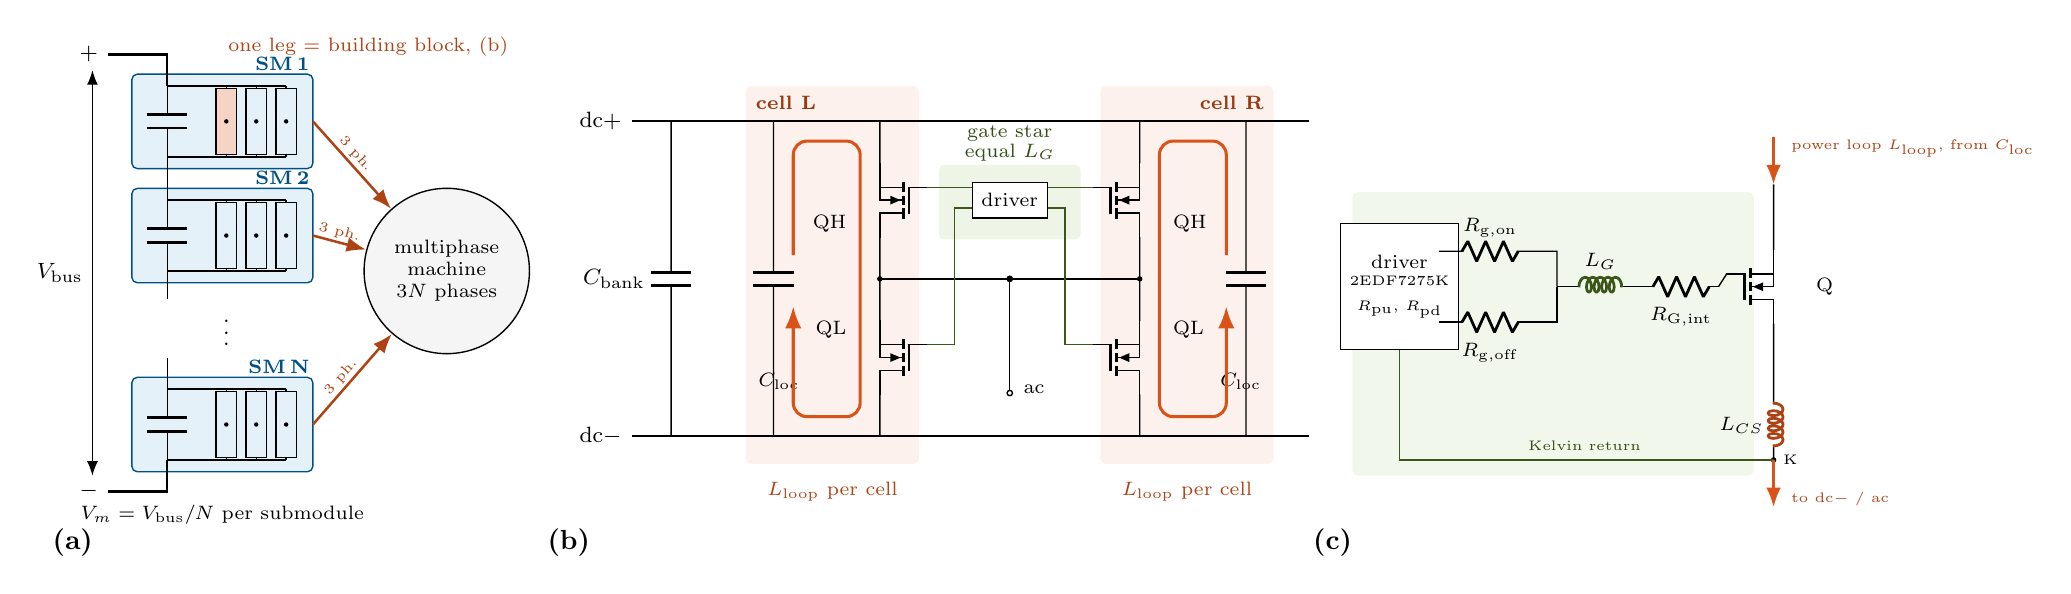
\begin{tikzpicture}[font=\footnotesize, >=Latex, line width=0.5pt]
\ctikzset{bipoles/length=0.85cm, tripoles/mos style/arrows}
\definecolor{cBlue}{rgb}{0.0,0.447,0.741}
\definecolor{cRed}{rgb}{0.85,0.325,0.098}
\definecolor{cGreen}{rgb}{0.466,0.674,0.188}
%------------------------------------------------------------------ (a) SPB
\begin{scope}
\node[draw, circle, minimum size=2.1cm, fill=gray!8, align=center, font=\scriptsize] (M) at (4.15,1.1)
  {multiphase\\machine\\$3N$ phases};
\foreach \k/\y/\lab in {1/3.0/1, 2/1.55/2, 3/-0.85/N}{
  \fill[cBlue!10, rounded corners=2pt] (0.15,\y-0.6) rectangle (2.45,\y+0.6);
  \draw[cBlue!70!black, rounded corners=2pt] (0.15,\y-0.6) rectangle (2.45,\y+0.6);
  \node[anchor=south east, cBlue!70!black, font=\scriptsize\bfseries, inner sep=1pt] at (2.45,\y+0.6) {SM\,\lab};
  \draw (0.6,\y+0.45) to[C] (0.6,\y-0.45);
  \draw (0.6,\y+0.45) -- (2.11,\y+0.45); \draw (0.6,\y-0.45) -- (2.11,\y-0.45);
  \foreach \j in {0,1,2}{
    \pgfmathsetmacro{\xx}{1.35+\j*0.38}
    \ifnum\k=1 \ifnum\j=0 \fill[cRed!25] (\xx-0.13,\y-0.42) rectangle (\xx+0.13,\y+0.42); \fi\fi
    \draw (\xx-0.13,\y-0.42) rectangle (\xx+0.13,\y+0.42);
    \draw (\xx,\y+0.42) -- (\xx,\y+0.45); \draw (\xx,\y-0.42) -- (\xx,\y-0.45);
    \fill (\xx,\y) circle (0.8pt);
  }
  \draw[cRed!80!black, ->, line width=0.9pt] (2.45,\y) -- ($(M.center)!1.06cm!(2.45,\y)$) node[pos=0.45, above, sloped, font=\tiny, inner sep=1pt]{3 ph.};
}
\node at (1.35,0.42) {$\vdots$};
\draw[thick] (0.6,3.45) -- (0.6,3.85) -- (-0.15,3.85) node[left]{$+$};
\draw[thick] (0.6,-1.30) -- (0.6,-1.7) -- (-0.15,-1.7) node[left]{$-$};
\draw (0.6,2.55) -- (0.6,2.0); \draw (0.6,1.1) -- (0.6,0.75); \draw (0.6,0.0) -- (0.6,-0.4);
\draw[<->] (-0.35,3.65) -- node[left, align=center]{$V_\mathrm{bus}$} (-0.35,-1.5);
\node[font=\scriptsize, align=left, cRed!80!black, anchor=west] at (1.25,3.95) {one leg = building block, (b)};
\node[font=\scriptsize, align=center] at (1.3,-2.0) {$V_m=V_\mathrm{bus}/N$ per submodule};
\node[font=\bfseries] at (-0.6,-2.35) {(a)};
\end{scope}
%------------------------------------------------------------------ (b) building block
\begin{scope}[xshift=7.1cm, yshift=-1.3cm]
\fill[cRed!8, rounded corners=2pt] (0.85,-0.05) rectangle (3.05,4.75);
\fill[cRed!8, rounded corners=2pt] (5.35,-0.05) rectangle (7.55,4.75);
\fill[cGreen!12, rounded corners=2pt] (3.3,2.8) rectangle (5.1,3.75);
\node[cRed!70!black, font=\scriptsize\bfseries, anchor=north west] at (0.85,4.75) {cell L};
\node[cRed!70!black, font=\scriptsize\bfseries, anchor=north east] at (7.55,4.75) {cell R};
\draw[thick] (-0.6,4.3) node[left]{dc$+$} -- (8.0,4.3);
\draw[thick] (-0.6,0.3) node[left]{dc$-$} -- (8.0,0.3);
\draw (-0.1,4.3) to[C, l_={$C_\mathrm{bank}$}] (-0.1,0.3);
% cell L
\draw (1.2,4.3) to[C] (1.2,0.3);
\node[font=\scriptsize, anchor=west] at (0.88,1.0) {$C_\mathrm{loc}$};
\draw (2.55,4.3) to[Tnigfete, n=QHL] (2.55,2.3) to[Tnigfete, n=QLL] (2.55,0.3);
\node[font=\scriptsize, anchor=east] at (2.25,3.0) {QH};
\node[font=\scriptsize, anchor=east] at (2.25,1.65) {QL};
% cell R
\draw (7.2,4.3) to[C] (7.2,0.3);
\node[font=\scriptsize, anchor=east] at (7.52,1.0) {$C_\mathrm{loc}$};
\draw (5.85,4.3) to[Tnigfete, n=QHR, mirror] (5.85,2.3) to[Tnigfete, n=QLR, mirror] (5.85,0.3);
\node[font=\scriptsize, anchor=west] at (6.15,3.0) {QH};
\node[font=\scriptsize, anchor=west] at (6.15,1.65) {QL};
% ac
\fill (2.55,2.3) circle (1pt); \fill (5.85,2.3) circle (1pt);
\draw (2.55,2.3) -- (5.85,2.3);
\draw (4.2,2.3) to[short, *-o] (4.2,0.85);
\node[font=\scriptsize, anchor=west] at (4.25,0.9) {ac};
% driver and gate star
\node[draw, fill=white, minimum width=0.95cm, minimum height=0.45cm, font=\scriptsize] (drv) at (4.2,3.3) {driver};
\draw[cGreen!50!black] (QHL.G) -- (QHL.G -| drv.west);
\draw[cGreen!50!black] (QHR.G) -- (QHR.G -| drv.east);
\draw[cGreen!50!black] (QLL.G) -| (3.5,3.2) -- (drv.west |- 0,3.2);
\draw[cGreen!50!black] (QLR.G) -| (4.9,3.2) -- (drv.east |- 0,3.2);
\node[font=\scriptsize, align=center, cGreen!45!black] at (4.2,4.02) {gate star\\[-1pt]equal $L_G$};
% commutation loops
\draw[cRed, line width=1.1pt, ->, rounded corners=5pt] (1.45,2.6) -- (1.45,4.05) -- (2.3,4.05) -- (2.3,0.55) -- (1.45,0.55) -- (1.45,1.95);
\draw[cRed, line width=1.1pt, ->, rounded corners=5pt] (6.95,2.6) -- (6.95,4.05) -- (6.1,4.05) -- (6.1,0.55) -- (6.95,0.55) -- (6.95,1.95);
\node[cRed!80!black, font=\scriptsize, align=center] at (1.95,-0.4) {$L_\mathrm{loop}$ per cell};
\node[cRed!80!black, font=\scriptsize, align=center] at (6.45,-0.4) {$L_\mathrm{loop}$ per cell};
\node[font=\bfseries] at (-1.4,-1.05) {(b)};
\end{scope}
%------------------------------------------------------------------ (c) gate and power circuit of one transistor
\begin{scope}[xshift=16.0cm, yshift=-1.3cm]
\fill[cGreen!10, rounded corners=2pt] (-0.35,-0.2) rectangle (4.75,3.4);
\node[draw, fill=white, minimum width=1.05cm, minimum height=1.6cm, align=center, font=\scriptsize] (D) at (0.25,2.2) {driver\\[-2pt]\tiny 2EDF7275K\\[1pt]\tiny $R_\mathrm{pu}$, $R_\mathrm{pd}$};
\draw (0.75,2.65) to[R, l={\scriptsize $R_\mathrm{g,on}$}] (2.05,2.65) -- (2.25,2.65) -- (2.25,2.2);
\draw (0.75,1.75) to[R, l_={\scriptsize $R_\mathrm{g,off}$}] (2.05,1.75) -- (2.25,1.75) -- (2.25,2.2);
\draw (2.25,2.2) to[L, l={\scriptsize $L_G$}, color=cGreen!50!black] (3.35,2.2) to[R, l_={\scriptsize $R_\mathrm{G,int}$}] (4.3,2.2);
\draw (5.0,3.5) to[Tnigfete, n=Q, mirror] (5.0,0.9);
\draw (4.3,2.2) -- (Q.G);
\draw (5.0,0.9) to[L, l_={\scriptsize $L_{CS}$}, color=cRed!80!black] (5.0,0.0);
\fill (5.0,0.0) circle (1pt) node[right, font=\tiny]{K};
\draw[cGreen!50!black] (5.0,0.0) -- (0.25,0.0) -- (D.south);
\node[font=\tiny, cGreen!45!black, anchor=south] at (2.6,0.0) {Kelvin return};
\draw[cRed, line width=0.9pt, ->] (5.0,0.0) -- (5.0,-0.6);
\draw[cRed, line width=0.9pt, <-] (5.0,3.5) -- (5.0,4.1);
\node[font=\tiny, cRed!80!black, anchor=west, align=left] at (5.1,3.95) {power loop $L_\mathrm{loop}$, from $C_\mathrm{loc}$};
\node[font=\tiny, cRed!80!black, anchor=west, align=left] at (5.1,-0.5) {to dc$-$ / ac};
\node[font=\scriptsize] at (5.65,2.2) {Q};

\node[font=\bfseries] at (-0.6,-1.05) {(c)};
\end{scope}
\end{tikzpicture}
}
\caption{(a) Stacked polyphase bridge (SPB) inverter: $N$ three-phase submodules (SM) are connected in series on the dc side and feed the $N$ three-phase winding sets of a multiphase machine; each submodule operates at $V_m=V_\mathrm{bus}/N$. (b) Building block designed in this paper, i.e., one phase leg of a submodule: two mirror-symmetric commutation cells (red) with one high-side (QH) and one low-side (QL) EPC2361 each, so that two transistors are paralleled per switch, local MLCCs $C_\mathrm{loc}$ in every cell, a common MLCC bank $C_\mathrm{bank}$ and a centre gate driver (green) with equal, star-connected gate loops. The red arrows indicate the commutation loop of each cell. (c) Gate and power circuit of one transistor: driver pull-up and pull-down resistances $R_\mathrm{pu}$, $R_\mathrm{pd}$, external gate resistors $R_\mathrm{g,on}$ and $R_\mathrm{g,off}$, gate-loop inductance $L_G$, internal gate resistance $R_\mathrm{G,int}$, and the common-source inductance $L_{CS}$ shared by the gate loop and the power loop up to the Kelvin connection K in the source pad. The values are given in Table~\ref{tab:para}.}
\label{fig:spb}
\end{figure*}

The target is a 1200\,V, 150\,kW traction inverter (Fig.~\ref{fig:spb}a). If the bus voltage $V_\mathrm{bus}$ is divided into $N$ submodules of $V_m=V_\mathrm{bus}/N$ that share the power equally, the power of one phase leg at modulation index $M$ and unity power factor is
\begin{equation}
P_\mathrm{leg}=\frac{M\,V_m}{2\sqrt2}\,I_\mathrm{ph},\qquad P=3N\,P_\mathrm{leg}=\frac{3M\,V_\mathrm{bus}}{2\sqrt2}\,I_\mathrm{ph},
\label{eq:pleg}
\end{equation}
so that the phase current $I_\mathrm{ph}$ is set by the inverter power and the bus voltage alone and is the same for every choice of $N$. With space-vector modulation ($M$\,=\,1.15), 150\,kW at 1200\,V requires about 100\,A$_\mathrm{rms}$ per phase. The phase current is therefore the fixed specification of the building block, whereas its voltage, the transistor and the number of submodules remain open and are chosen in the procedure of Fig.~\ref{fig:flow}: the voltage class and the transistor first (Section~\ref{sec:vclass}), then the layout and gate-drive concept, which determines how transistors can be paralleled (Section~\ref{sec:layout}), the number of paralleled devices (Section~\ref{sec:npar}) and the dc link (Section~\ref{sec:dclink}); the parasitics, switching energies, losses and temperatures are then verified with one parametric geometry that drives the PCB placement, an Ansys Q3D extraction, LTspice, a frequency-domain copper-loss model and an Ansys Icepak model (Sections~\ref{sec:para}--\ref{sec:thermal}).

\begin{figure*}[t]
\centering
\resizebox{\textwidth}{!}{% Fig. 2: design procedure of the SPB building block (\input from spb_bb_ieee.tex; standalone: fig_flow_standalone.tex)
\begin{tikzpicture}[font=\footnotesize, >=Latex, line width=0.5pt,
  stp/.style={draw, fill=white, align=center, minimum width=3.6cm, minimum height=0.5cm, inner sep=1.5pt, font=\scriptsize},
  res/.style={stp, fill=gray!20},
  inp/.style={draw, fill=white, trapezium, trapezium left angle=75, trapezium right angle=105, align=center,
              minimum height=0.45cm, inner sep=1pt, font=\scriptsize},
  dec/.style={draw, fill=white, diamond, aspect=2.6, align=center, inner sep=0.5pt, font=\scriptsize},
  sub/.style={draw, rounded corners=1.5pt, fill=white},
  ttl/.style={font=\small\bfseries, anchor=north west, inner sep=2pt},
  sec/.style={font=\scriptsize, text=red!75!black}]
\definecolor{cA}{rgb}{0.0,0.40,0.75}\definecolor{cB}{rgb}{0.15,0.55,0.15}
\definecolor{cC}{rgb}{0.85,0.30,0.10}\definecolor{cD}{rgb}{0.45,0.20,0.60}\definecolor{cV}{rgb}{0.80,0.50,0.0}
% ---------------- specification
\definecolor{cM}{rgb}{0.55,0.35,0.10}
\node[draw, thick, minimum width=8.6cm, minimum height=1.25cm, align=center, fill=gray!6] (spec) at (4.3,13.8)
 {\normalsize SPB traction inverter specification\\[1pt]
  $P$\,=\,150\,kW, $V_\mathrm{bus}$\,=\,1200\,V, $M\leq1.15$, $\eta\geq99.5$\,\%, $T_{j,\max}$\\[1pt]
  $\Rightarrow$ $I_\mathrm{ph}$\,=\,100\,A$_\mathrm{rms}$ for any number of submodules $N$};
\node[draw, thick, cM, minimum width=8.6cm, minimum height=1.25cm, align=center, fill=cM!8, text=black] (mach) at (13.5,13.8)
 {\normalsize\color{cM}$\square$ Machine side (multiphase, $N$ winding sets)\\[1pt]
  ripple $\Delta i\propto V_m/(L_\sigma f_\mathrm{sw})$, winding step $V_m$, $dv/dt$, $R_\mathrm{ac}(f)$\\[1pt]
  $\Rightarrow$ $N$, $V_m$, $f_\mathrm{sw}$; integration: space, coolant, end winding};
\draw[<->, thick, cM] (spec.east) -- (mach.west);
% ---------------- four selection modules
\foreach \x/\c/\n in {0/cA/A, 4.6/cB/B, 9.2/cC/C, 13.8/cD/D}{
  \draw[\c, thick, rounded corners=3pt, fill=\c!4] (\x,5.4) rectangle ++(4.0,6.6);
}
\draw[->, thick] (2.0,13.17) -- (2.0,12.0); \draw[->, thick] (6.0,13.17) -- (6.0,12.0);
\draw[->, thick, cM] (10.6,13.17) -- node[right, font=\tiny, pos=0.12]{$f_\mathrm{sw}$} (10.6,12.0);
\draw[->, thick, cM] (15.8,13.17) -- node[right, font=\tiny, pos=0.12]{$f_\mathrm{sw}$, ripple} (15.8,12.0);
\draw[->, thick, cM] (9.4,13.17) |- (3.0,12.9) -- (3.0,12.0);
\node[font=\tiny, text=cM, anchor=south] at (4.5,12.9) {$N$, $V_m$};
% A: voltage class and device
\node[ttl, text=cA] at (0,12.0) {$\square$ Voltage class \& device};
\node[inp] (a1) at (2.0,11.1) {GaN datasheets\\[-1pt]$R_\mathrm{DS(on)}$, $Q_\mathrm{oss}$, $V_\mathrm{DS}$};
\node[stp] (a2) at (2.0,10.35) {classes 100, 200, 350, 650\,V\\[-1pt]$V_m$, $N=V_\mathrm{bus}/V_m$};
\node[stp] (a3) at (2.0,9.5) {$P_\mathrm{min}=6IV_\mathrm{bus}\sqrt{f_\mathrm{sw}\tau}$\\[-1pt]$\tau=R_\mathrm{DS(on)}C_\mathrm{oss,tr}$};
\node[res] (a4) at (2.0,8.55) {EPC2361, $V_m$\,=\,75\,V, $N$\,=\,16};
\draw[->] (a1) -- (a2); \draw[->] (a2) -- (a3); \draw[->] (a3) -- (a4);
\node at (2.0,6.85) {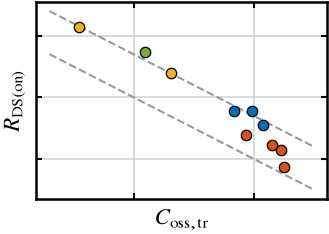
\includegraphics[width=2.6cm]{devices.png}};
\node[sec] at (2.0,5.62) {Section III};
% B: layout and gate-drive concept
\node[ttl, text=cB] at (4.6,12.0) {$\square$ Layout \& gate drive};
\node[stp] (b1) at (6.6,11.05) {sharing sensitivity, 2 FETs\\[-1pt]$L_G$, $L_{CS}$, $L_D$, $V_\mathrm{th}$ (LTspice)};
\node[stp] (b2) at (6.6,10.2) {equal $L_G$ and $L_{CS}$:\\[-1pt]star driver per FET pair, Kelvin};
\node[stp] (b3) at (6.6,9.35) {two mirrored cells,\\[-1pt]vertical loops on L1/L2};
\node[res] (b4) at (6.6,8.55) {cell + driver concept, scaling};
\draw[->] (b1) -- (b2); \draw[->] (b2) -- (b3); \draw[->] (b3) -- (b4);
\node at (6.6,6.85) {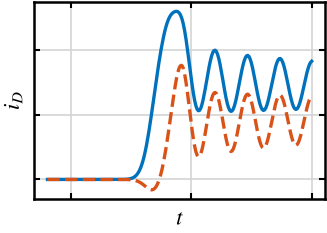
\includegraphics[width=2.6cm]{sharing.png}};
\node[sec] at (6.6,5.62) {Section IV};
% C: number of devices in parallel
\node[ttl, text=cC] at (9.2,12.0) {$\square$ Devices in parallel};
\node[stp] (c1) at (11.0,11.05) {$n$\,=\,1, 2, 3, 4 per switch};
\node[stp] (c2) at (11.0,10.4) {$P_\mathrm{cond}\propto1/n$, $P_\mathrm{sw}(n)$, $P_\mathrm{Cu}$};
\node[dec] (c3) at (11.0,9.45) {loss gain vs.\\[-1pt]drivers $n_\mathrm{drv}$?};
\node[res] (c4) at (11.0,8.55) {$n$\,=\,2 (one driver)};
\draw[->] (c1) -- (c2); \draw[->] (c2) -- (c3); \draw[->] (c3) -- node[right, font=\tiny]{} (c4);
\draw[->] (c3.east) -- ++(0.25,0) |- node[pos=0.25, right, font=\tiny]{$n{+}1$} (c1.east);
\node at (11.0,6.85) {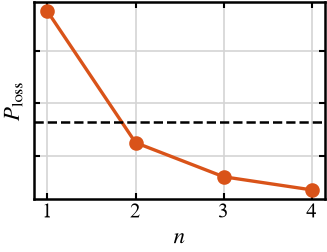
\includegraphics[width=2.6cm]{npar.png}};
\node[sec] at (11.2,5.62) {Section V};
% D: dc link
\node[ttl, text=cD] at (13.8,12.0) {$\square$ DC-link capacitors};
\node[stp, minimum width=1.7cm] (d1) at (14.85,11.05) {$\Delta v_\mathrm{pp}\rightarrow C_v$};
\node[stp, minimum width=1.7cm] (d2) at (16.75,11.05) {$I_{C,\mathrm{rms}}\rightarrow C_i$};
\node[stp] (d3) at (15.8,10.35) {$C_\mathrm{dc}=\max\{C_v,\,C_i\}$};
\node[stp] (d4) at (15.8,9.55) {MLCC: $C(V_\mathrm{dc})$, ESR, ESL,\\[-1pt]local + bank hierarchy};
\node[res] (d5) at (15.8,8.55) {24$\times$1210 + 12$\times$0805};
\draw[->] (d1) -- (d1 |- d3.north); \draw[->] (d2) -- (d2 |- d3.north); \draw[->] (d3) -- (d4); \draw[->] (d4) -- (d5);
\node at (15.8,6.85) {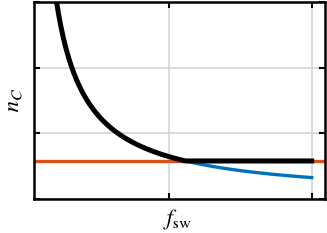
\includegraphics[width=2.6cm]{dclink.png}};
\node[sec] at (15.8,5.62) {Section VI};
% module chain
\draw[->, thick] (4.0,8.55) -- (4.6,8.55); \draw[->, thick] (8.6,8.55) -- (9.2,8.55); \draw[->, thick] (13.2,8.55) -- (13.8,8.55);
% ---------------- verification
\draw[cV, thick, rounded corners=3pt, fill=cV!5] (0,0.1) rectangle (13.4,4.95);
\node[ttl, text=cV!90!black] at (0,4.95) {$\square$ Verification with one parametric geometry};
\node[sec, anchor=north east] at (13.4,4.95) {Sections VII--XI};
\foreach \x/\t/\img/\o [count=\k] in {
  0.15/PCB placement/kicad_3d.png/{KiCad, 3D models},
  2.37/Q3D extraction/q3d_model.png/{$R(f)$, $L(f)$, $L_\mathrm{loop}$, $L_G$, $L_{CS}$},
  4.59/LTspice/switching.png/{$E_\mathrm{on}$, $E_\mathrm{off}$, $R_G$, $\hat V_\mathrm{DS}$, gate bump},
  6.81/Loss model/losses.png/{cond., sw., Cu($f$), MLCC},
  9.03/Icepak/icepak_model.png/{$T_j$, $T_\mathrm{PCB}$, cooling},
  11.25/Cell assembly/cell_iso.png/{cold plate, busbar, insulation, leads}}{
  \node[sub, minimum width=2.0cm, minimum height=3.75cm, anchor=south west] (v\k) at (\x,0.45) {};
  \node[font=\scriptsize\bfseries, anchor=north] at (\x+1.0,4.15) {\t};
  \node at (\x+1.0,2.6) {\includegraphics[width=1.85cm, height=1.75cm, keepaspectratio]{\img}};
  \node[font=\tiny, align=center, text width=1.95cm] at (\x+1.0,0.95) {\o};
}
\foreach \a/\b in {1/2, 2/3, 3/4, 4/5, 5/6} \draw[->, thick] (v\a.east) -- (v\b.west);

% inputs from the modules
\draw[->, cA] (2.0,5.4) -- node[right, font=\tiny]{EPC2361 model, $V_m$} (2.0,4.95);
\draw[->, cB] (6.6,5.4) -- node[right, font=\tiny]{geometry, driver} (6.6,4.95);
\draw[->, cC] (11.2,5.4) -- node[right, font=\tiny]{$n$} (11.2,4.95);
\draw[->, cD] (15.8,5.4) -- (15.8,5.15) -- node[above, font=\tiny, pos=0.6]{$C$, ESR, ESL} (12.6,5.15) -- (12.6,4.95);
% ---------------- decision and outcome
\node[dec, minimum width=3.6cm] (q) at (15.8,3.05) {$\hat V_\mathrm{DS}$, $\eta$, $T_j$, sharing,\\[-1pt]machine loss met?};
\draw[->, thick] (13.4,3.05) -- (q.west);
\node[draw, dashed, fill=gray!10, align=center, minimum width=3.6cm, minimum height=0.85cm, font=\scriptsize] (hw) at (15.8,0.6)
  {prototype: double pulse,\\[-1pt]continuous, motor (future work)};
\draw[->, thick] (q.south) -- node[right, font=\scriptsize]{yes} (hw.north);
\draw[->, thick, red!70!black] (q.east) -- (18.15,3.05) -- node[pos=0.55, above, sloped, font=\scriptsize]{no: modify layout, $R_G$, $n$, $C_\mathrm{dc}$, $f_\mathrm{sw}$} (18.15,12.45) -- (7.0,12.45) -- (7.0,12.0);
\end{tikzpicture}
}
\caption{Design procedure of the SPB building block. From the inverter specification, four selection steps fix the voltage class and transistor (Section~\ref{sec:vclass}), the layout and gate-drive concept (Section~\ref{sec:layout}), the number of paralleled devices (Section~\ref{sec:npar}) and the dc-link capacitors (Section~\ref{sec:dclink}). The machine side (top right) feeds back the number of winding sets $N$, the submodule voltage $V_m$ and, through the current ripple, the switching frequency (Section~\ref{sec:integ}). One parametric geometry then drives the PCB placement, the Q3D extraction, the LTspice switching model, the loss model with frequency-dependent copper resistance, the Icepak model and the cell assembly (Sections~\ref{sec:para}--\ref{sec:integ}); if the overshoot, efficiency, temperature or sharing targets are missed, the layout, gate resistors, device count dc link or switching frequency are modified. The thumbnails show results of the respective steps.}
\label{fig:flow}
\end{figure*}

%=========================================================================
\section{Voltage Class and Transistor}\label{sec:vclass}
%=========================================================================
The submodule voltage, and with it the transistor voltage class, is the first design decision. Every submodule carries the same phase current $I$ independent of $N$, see~\eqref{eq:pleg}. With $n$ transistors per switch, the conduction loss of all submodules scales with $NI^2R_\mathrm{DS(on)}/n$ and the loss associated with the output charge with $Nnf_\mathrm{sw}Q_\mathrm{oss}V_m$. With $Q_\mathrm{oss}\approx C_\mathrm{oss,tr}V_m$ and an optimal number of devices, $n^\ast=I\sqrt{R_\mathrm{DS(on)}/(f_\mathrm{sw}Q_\mathrm{oss}V_m)}$, the sum of the two over all three legs of all submodules becomes
\begin{equation}
P_\mathrm{min}=6\,I\,V_\mathrm{bus}\sqrt{f_\mathrm{sw}\,R_\mathrm{DS(on)}C_\mathrm{oss,tr}} .
\label{eq:pmin}
\end{equation}
To first order the voltage class cancels, and candidates are ranked by the device time constant $\tau=R_\mathrm{DS(on)}C_\mathrm{oss,tr}$, a hard-switching device figure of merit (D-FOM) for the SPB.

\begin{figure*}[t]
\centering
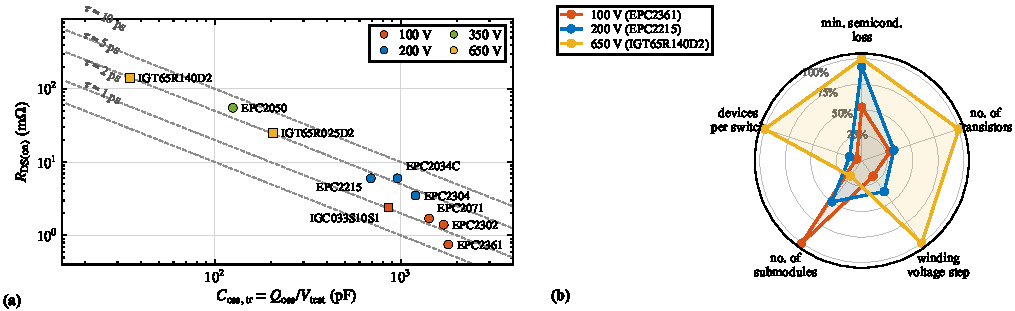
\includegraphics[width=0.92\textwidth]{fig_devices.pdf}
\caption{Voltage-class selection for a 1200\,V SPB with 100\,A$_\mathrm{rms}$ phase current at 50\,kHz. (a) Typical on-resistance at 25\,$^\circ$C against the time-related output capacitance $C_\mathrm{oss,tr}=Q_\mathrm{oss}/V_\mathrm{test}$ of off-the-shelf GaN transistors (circles: EPC, squares: Infineon; datasheet values), with lines of constant device time constant $\tau=R_\mathrm{DS(on)}C_\mathrm{oss,tr}$. (b) Comparison of SPBs built from the best device of the 100, 200 and 650\,V classes, each axis normalized to its maximum: minimum conduction plus output-charge loss~\eqref{eq:pmin}, optimum number of devices per switch $n^\ast$, number of submodules $N$, voltage step at the winding $V_m$ and total number of transistors $6Nn^\ast$.}
\label{fig:devices}
\end{figure*}

\begin{table}[t]
\centering
\caption{Off-the-Shelf GaN Transistors for a 1200\,V SPB (100\,A$_\mathrm{rms}$, 50\,kHz)}
\label{tab:devices}
\setlength{\tabcolsep}{2.5pt}
\resizebox{\columnwidth}{!}{%
\begin{tabular}{@{}lccccccc@{}}
\toprule
Device & $V_\mathrm{DS}$ & $R_\mathrm{DS(on)}$ & $C_\mathrm{oss,tr}$ & $V_m$ & $\tau$ & $N$ & $P_\mathrm{min}$ \\
 & [V] & [m$\Omega$] & [pF] & [V] & [ps] & & rel. \\
\midrule
\DeviceRows
\bottomrule
\end{tabular}}
\end{table}

Fig.~\ref{fig:devices} and Table~\ref{tab:devices} compare ten EPC and Infineon devices from the 100, 200, 350 and 650\,V classes, each operated at a submodule voltage of 60--75\,\% of its rating, i.e., with 16, 8, 5 and 3 submodules. The 100\,V devices reach $\tau$\,=\,\TauEPC--2.4\,ps, the 200\,V devices \TauBestTwo--5.8\,ps, the only available 350\,V device \TauBestThree\,ps and the 650\,V devices about \TauBestSix\,ps. An SPB built from EPC2361 therefore has a \PminTwo\ times lower minimum loss than one built from the best 200\,V device and a \PminSix\ times lower one than with 650\,V devices. Three practical arguments point the same way. First, at 100\,A per submodule the optimum number of high-voltage devices per switch becomes impractical (\NoptIGT\ for IGT65R025D2), whereas EPC2361 needs about \NoptEPC; the overlap and copper losses, not included in~\eqref{eq:pmin}, reduce this further (Section~\ref{sec:npar}). Second, the 3\,$\times$\,5\,mm packages of the 100\,V class allow sub-nanohenry commutation loops (Section~\ref{sec:para}). Third, the on-resistance of the 650\,V devices rises by a factor of 2.1 at 150\,$^\circ$C, against 1.8 for EPC2361. The price is a larger number of submodules, i.e., more gate drivers, auxiliary supplies and control channels, which the modularity of the SPB accommodates~\cite{jin2017}. This contrasts with the 650\,V GaN SPB of~\cite{rohner2024}, where the submodule count rather than the device figure of merit was minimized. The 100\,V class and EPC2361 (0.75\,m$\Omega$ typical, 3\,$\times$\,5\,mm) are therefore selected.

With 100\,V transistors, 16 submodules give a nominal submodule voltage of 75\,V. The submodule voltage may rise to 90\,V with battery-voltage variation and unbalance between submodules, which leaves 10\,V to the rating for overshoot and ringing; the peak drain--source voltage must therefore stay below 90\,V at the maximum current. From~\eqref{eq:pleg}, one leg delivers \Prated\,kW at $M$\,=\,1 and \Pmax\,kW at $M$\,=\,1.15, i.e., about 9.2\,kW per submodule and 146\,kW for the inverter. Table~\ref{tab:key} summarizes the resulting specification of the building block together with the design decisions and results of the following sections. Using the device power utilization of~\cite{cooke2026}, $\mathrm{DPU}=V_\mathrm{dc}I_\mathrm{ph}R_\mathrm{DS(on)}/(nV_\mathrm{DS}^2)\cdot10^4$, the block is rated at a DPU of \DpuMax{}, comparable to the continuously operated paralleled-GaN inverters reviewed in~\cite{cooke2026} (2.3--9.5).

\begin{table}[t]
\centering
\caption{Building-Block Specification, Design and Key Results}
\label{tab:key}
\setlength{\tabcolsep}{4pt}
\resizebox{\columnwidth}{!}{%
\begin{tabular}{@{}ll@{}}
\toprule
\multicolumn{2}{@{}l}{\textbf{Specification (1200\,V, 150\,kW SPB, $N$\,=\,16)}} \\
Submodule voltage nominal / max. & 75\,V / 90\,V \\
Phase current & 100\,A$_\mathrm{rms}$ (\Ipk\,A peak) \\
Power per leg ($M$\,=\,1 / 1.15) & \Prated\,/\,\Pmax\,kW \\
Targets & $\eta\geq99.5$\,\%, $\hat V_\mathrm{DS}<90$\,V at 160\,A \\
\midrule
\multicolumn{2}{@{}l}{\textbf{Design}} \\
Transistors & 2\,$\times$\,EPC2361 (100\,V, 0.75\,m$\Omega$) per switch \\
Gate drive & 2EDF7275K, +5/$-$1\,V, star-connected gates \\
Board & 30\,$\times$\,28.2\,mm, 4 layers, 2\,oz, 0.1\,mm L1--L2 \\
DC link per leg & 24\,$\times$\,10\,\uF{} 1210 + 12\,$\times$\,1\,\uF{} 0805 MLCC \\
$R_\mathrm{g,on}/R_\mathrm{g,off}$ (external) & \RgOn/\RgOff\,$\Omega$ (3.0/0.8\,$\Omega$ total) \\
\midrule
\multicolumn{2}{@{}l}{\textbf{Results (simulation)}} \\
Commutation loop per cell (Q3D) & \LloopCu\,nH copper, \LloopEsl\,nH with ESL \\
Gate loop per transistor (Q3D) & \LgateOne\,nH, equal for all four \\
Peak $V_\mathrm{DS}$ at 160\,A (HS/LS) & \VdsH\,/\,\VdsL\,V \\
Loss / efficiency at 50\,kHz & \Ptot\,W / \Eta\,\% \\
$T_j$ at 60\,$^\circ$C cold plate & \ThFetTop\,$^\circ$C (\ThFetBoth\,$^\circ$C with bottom pad) \\
\bottomrule
\end{tabular}}
\end{table}

%=========================================================================
\section{Layout and Gate-Drive Concept}\label{sec:layout}
%=========================================================================
Before the number of paralleled devices can be chosen, the way in which transistors are paralleled must be fixed, because it determines both the current sharing and the auxiliary circuits. Paralleled GaN transistors share the conduction loss well, since the on-resistance has a positive temperature coefficient, but not necessarily the switching loss: a transistor whose gate loop is longer, or whose common-source inductance differs, turns on later and off earlier than its neighbor and takes a larger part of the switching energy~\cite{lu2017,tran2025}. How strongly the layout asymmetry matters is quantified with an LTspice double-pulse model of two paralleled EPC2361 at 75\,V and 120\,A, in which one asymmetry is introduced at a time (Fig.~\ref{fig:sharing}). With a symmetric layout and Kelvin source connections both transistors carry the same current and energy. A gate-loop mismatch of 2 versus 8\,nH delays the second gate by about 2\,ns, half of the 4\,ns current rise, and gives a dynamic imbalance of 19\,\% with a 4:1 split of the turn-on energy (Fig.~\ref{fig:sharing}a.ii). Without Kelvin connections, a symmetric common-source inductance only slows both transistors, but a 0.2\,nH mismatch of it is the worst case, with 29\,\% imbalance and 2.8 times the turn-on energy in one device (a.iii). A threshold-voltage spread of 0.3\,V gives 7\,\% at turn-on but a 2:1 split of the turn-off energy, and a 0.3\,nH drain-path mismatch only 2\,\%. The static sharing at the end of the pulse is 59--60\,A per device in every case, since it is set by $R_\mathrm{DS(on)}$. Asymmetric switching therefore concentrates the switching loss in one device, which then sets the thermal limit of the whole switch; the layout must make the gate loops and the common-source paths equal, whereas the power-loop paths are less critical.

\begin{figure*}[t]
\centering
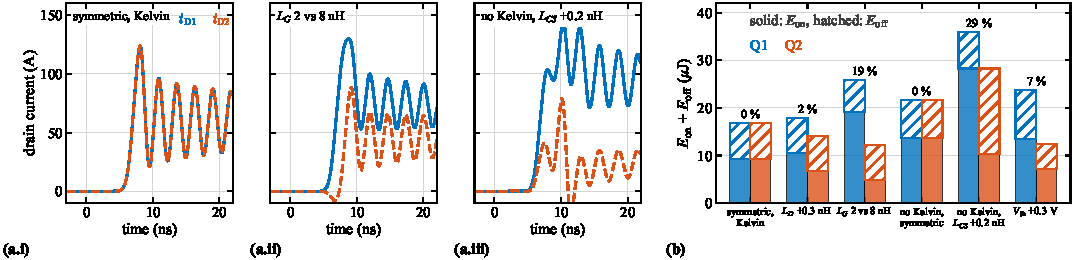
\includegraphics[width=0.92\textwidth]{fig_sharing.pdf}
\caption{Sensitivity of the current sharing of two paralleled EPC2361 (LTspice, low-side double pulse, 75\,V, 120\,A, $R_G$\,=\,2\,$\Omega$, baseline $L_G$\,=\,2\,nH, $L_D$\,=\,0.15\,nH, $L_S$\,=\,0.05\,nH). (a) Drain currents at turn-on for (a.i) the symmetric layout with Kelvin connections, (a.ii) a gate-loop mismatch of 2 versus 8\,nH and (a.iii) no Kelvin connection with a common-source inductance mismatch of 0.2\,nH. (b) Turn-on (solid) and turn-off (hatched) energy of the two transistors for one asymmetry at a time, with the dynamic current imbalance $(i_1-i_2)/(i_1+i_2)$ at the turn-on peak.}
\label{fig:sharing}
\end{figure*}

The building block therefore uses one dual-channel isolated gate driver (2EDF7275K, one channel per switch, split +5/$-$1\,V supply, Section~\ref{sec:para}) for every pair of paralleled transistors, placed on the symmetry line between them and connected to both gates in a star with Kelvin source returns, so that both gate loops are equal by construction. The power stage is split accordingly into two mirror-symmetric commutation cells, each with one high-side and one low-side transistor and its own local capacitors (Fig.~\ref{fig:spb}b). The concept scales in pairs (Fig.~\ref{fig:npar}a): one driver serves one or two devices per switch; three devices per switch need a second driver, since a third branch cannot be made equal to the other two, and four devices per switch are built as two of the two-device structures with two drivers. The number of drivers, and with them the isolated auxiliary supplies, level shifters and control channels, thus doubles from two to three devices per switch.

\begin{figure*}[t]
\centering
\subfloat[]{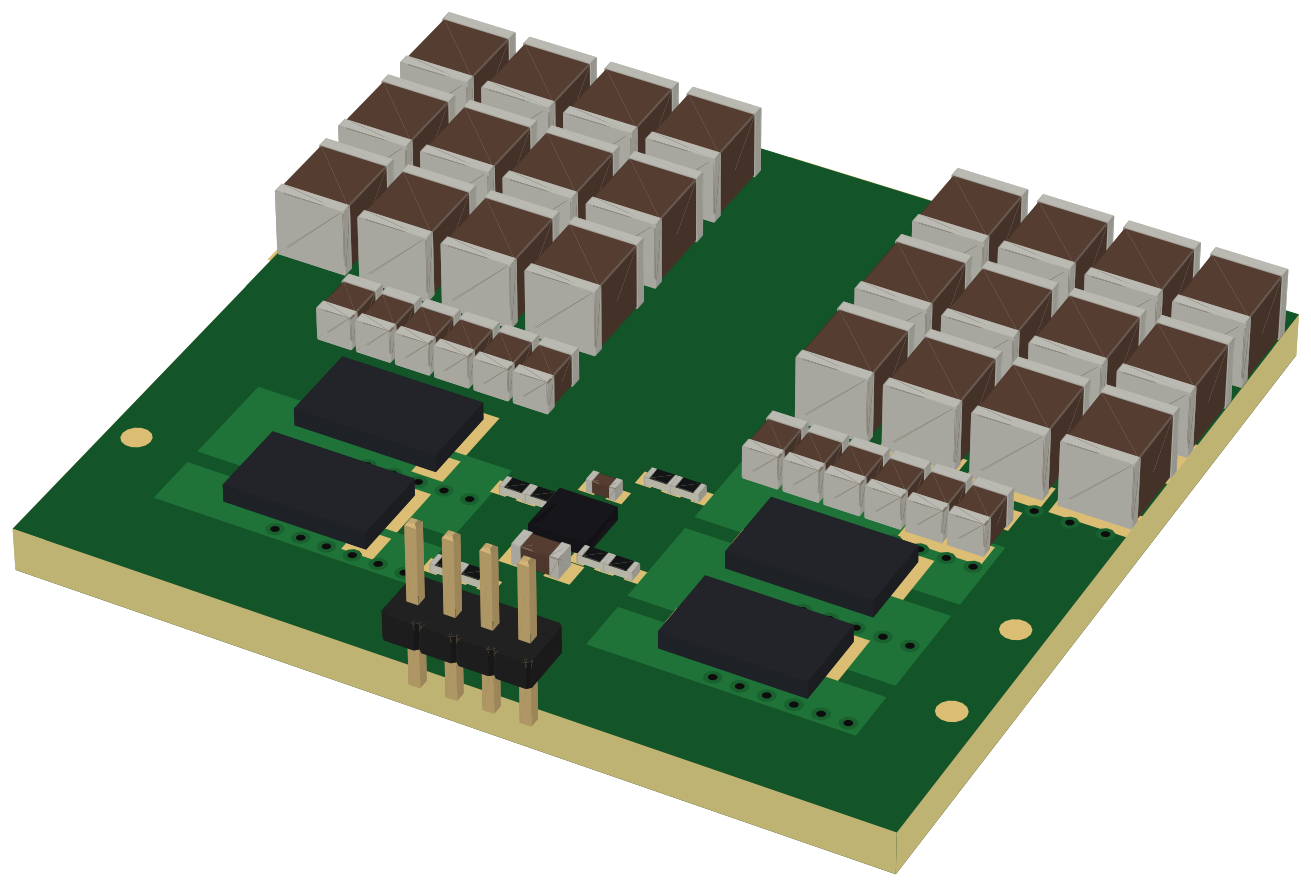
\includegraphics[height=2.7cm]{kicad_3d.png}}\hfill
\subfloat[]{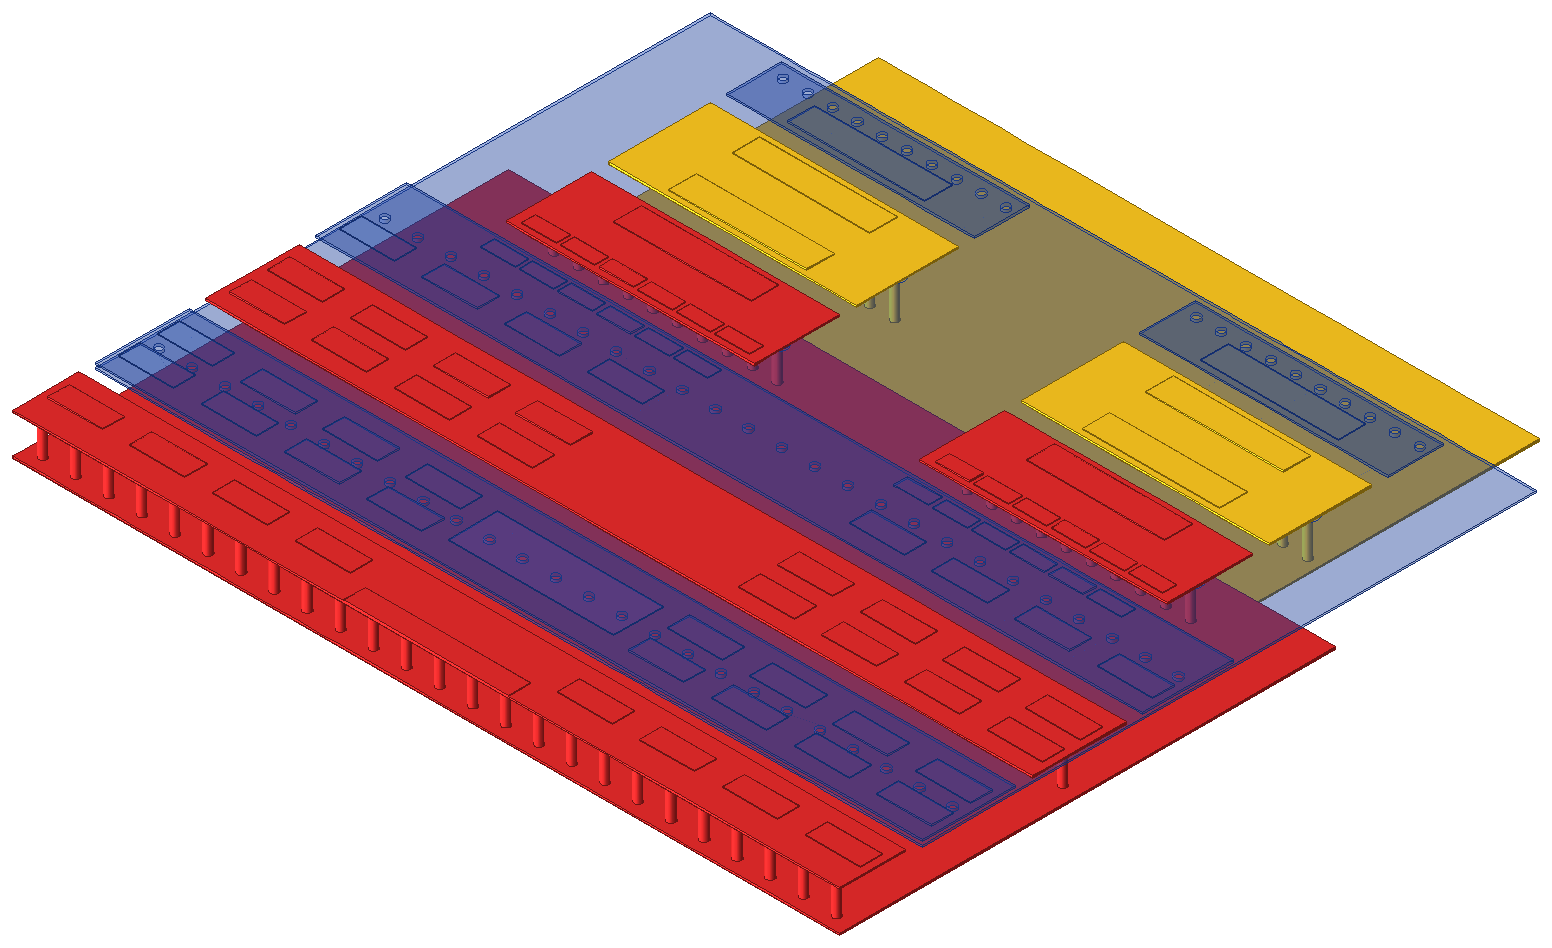
\includegraphics[height=2.5cm]{q3d_model.png}}\hfill
\subfloat[]{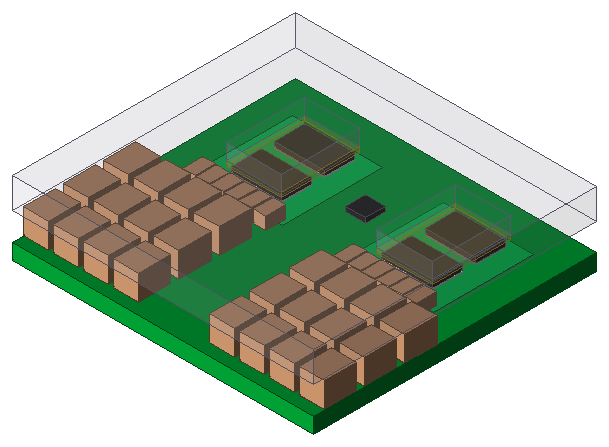
\includegraphics[height=2.7cm]{icepak_model.png}}
\caption{One parametric geometry, three models. (a) KiCad placement with the component 3D models (30\,$\times$\,28.2\,mm, four layers, 2\,oz copper): MLCC bank (top), local MLCCs, the two mirrored cells with QH and QL, and the centre driver. (b) Ansys Q3D copper model with the dc$+$ (red), dc$-$ (blue, transparent) and ac (yellow) nets and the via rows of the vertical loops. (c) Ansys Icepak model with gap pads, pedestals and the aluminium cold plate (shown above the board).}
\label{fig:layout}
\end{figure*}

In each cell the commutation loop is vertical: the forward path on layer L1 is closed on the dc$-$ plane on L2, 0.1\,mm below, so that the opposing currents cancel their flux. The dc$+$ plane on L3 and the ac plane on L4 carry the load current to the terminals on the symmetry line, and the capacitor bank above the cells feeds both cells equally, which avoids the shared, cascaded loop inductance identified in~\cite{brothers2019}. The driver sits in the 6\,mm corridor between the cells. The board measures 30\,$\times$\,28.2\,mm (\Area\,cm$^2$, \PdArea\,kW/cm$^2$ at board level). The same parametric geometry generates the KiCad placement, the Q3D model and the Icepak model (Fig.~\ref{fig:layout}), so that a change of, e.g., the prepreg thickness propagates to the inductances, losses and temperatures without manual steps.

%=========================================================================
\section{Number of Devices in Parallel}\label{sec:npar}
%=========================================================================
\begin{figure*}[t]
\centering
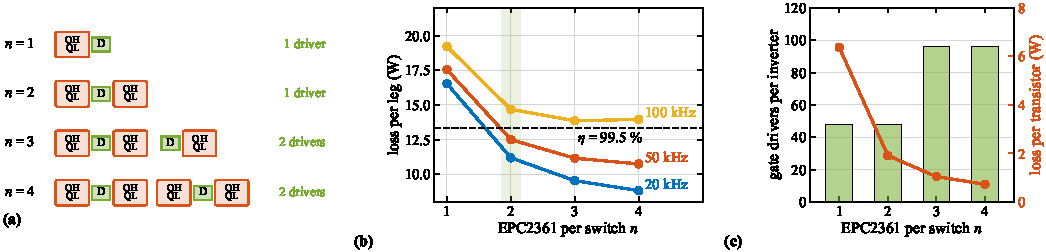
\includegraphics[width=0.92\textwidth]{fig_npar.pdf}
\caption{Number of EPC2361 per switch. (a) Scaling of the layout concept: two-device cells (red) with one star-connected half-bridge driver (D, green) per pair; three devices per switch need a second driver, four are built from two two-device structures. (b) Loss per leg at the rated point (75\,V, 100\,A$_\mathrm{rms}$, $M$\,=\,1, typical $R_\mathrm{DS(on)}$ at 100\,$^\circ$C, including copper and capacitor losses) for 20, 50 and 100\,kHz; the dashed line is the 99.5\,\% target. (c) Gate drivers of the complete 1200\,V inverter (16 submodules, 48 legs) and loss per transistor at 50\,kHz.}
\label{fig:npar}
\end{figure*}

The number of transistors per switch $n$ trades the conduction loss, which falls with $1/n$, against the current-independent part of the switching energy, which grows with $n$, and against the number of drivers. Fig.~\ref{fig:npar}(b) evaluates the leg loss with the switching energies of Section~\ref{sec:sw} and the copper and capacitor losses of Sections~\ref{sec:dclink} and~\ref{sec:loss}. One device per switch misses the efficiency target at all frequencies (\TotNone\,W at 50\,kHz, \PdevNone\,W per device, which is also difficult to cool through a 3\,$\times$\,5\,mm package). The step from one to two devices removes \CondNone{}$-$\CondNtwo\,W of conduction loss and reduces the leg loss to \TotNtwo\,W (\EtaNtwo\,\%) and the device loss to \PdevNtwo\,W. Three and four devices reduce the leg loss by only a further 1.3 and 1.7\,W, because the conduction loss is already smaller than the copper loss and the output-charge loss grows (\SwNtwo, \SwNthree{} and \SwNfour\,W switching loss for two, three and four devices). At the same time, three devices per switch double the number of gate drivers from 48 to 96 in the complete inverter (Fig.~\ref{fig:npar}c), together with their isolated supplies and signal channels, and lengthen the loops. Two devices per switch, i.e., two cells with one centre driver, are therefore selected.

%=========================================================================
\section{DC-Link Capacitor Design}\label{sec:dclink}
%=========================================================================
Each submodule needs its own dc link, which must (i) limit the switching-frequency voltage ripple, (ii) carry the ripple current of the legs, (iii) close the commutation loops with a minimum of inductance and (iv) fit on the building block. With three legs on one submodule bus, the high-frequency capacitor current of one leg is 28.8\,A$_\mathrm{rms}$ at the rated point and up to 50\,A$_\mathrm{rms}$ at low modulation index and zero power factor; limiting the peak-to-peak ripple to 4\,\% (3\,V) at 50\,kHz requires an effective capacitance of \CreqBlock\,\uF{} per leg, compared with \CreqAlone\,\uF{} if one leg had to supply its own ripple.

Film capacitors avoid the dc-bias loss of capacitance but need several times the volume at 100\,V and add lead inductance, and electrolytic or polymer capacitors cannot carry this ripple current per volume at 50\,kHz and above. Class-II MLCCs are therefore used, in two levels (Fig.~\ref{fig:spb}b, Table~\ref{tab:caps}). Six 1\,\uF{} 0805 capacitors per cell sit directly at the high-side drain and define the commutation loop, and a bank of 24 10\,\uF{} 1210 capacitors in three rows above the cells supplies the ripple charge. Because the capacitance of X7S dielectrics falls strongly with dc bias, the effective values at 75\,V are taken as 30\,\% (1210) and 45\,\% (0805) of the nominal values, which gives \CeffBlock\,\uF{} per leg and meets the ripple requirement at 50\,kHz. Fig.~\ref{fig:dclink}(a) shows that the number of bank capacitors is set by the voltage ripple up to about \Fcross\,kHz and by the ripple current per capacitor above, where raising the switching frequency no longer reduces the dc-link size.

\begin{table}[t]
\centering
\caption{DC-Link Capacitors per Leg (75\,V, 50\,kHz, Rated Point)}
\label{tab:caps}
\setlength{\tabcolsep}{3pt}
\resizebox{\columnwidth}{!}{%
\begin{tabular}{@{}lcc@{}}
\toprule
 & local (per cell) & bank \\
\midrule
Part & TDK C2012X7S2A105K125AB & Murata GRM32EC72A106KE05L \\
Size, dielectric & 0805, X7S, 100\,V & 1210, X7S, 100\,V \\
Number per leg & 2\,$\times$\,6 & 24 (3 rows of 8) \\
$C_\mathrm{nom}$ / $C_\mathrm{eff}$ at 75\,V$^\ast$ & 1\,\uF{} / 0.45\,\uF{} & 10\,\uF{} / 3.0\,\uF{} \\
ESR$^\ast$ / ESL$^\ast$ per part & 6\,m$\Omega$ / 0.48\,nH & 3\,m$\Omega$ / 0.5\,nH \\
Self-resonance & 10.8\,MHz & 4.1\,MHz \\
Ripple current per part (network) & 1.1\,A$_\mathrm{rms}$ & 2.0--2.1\,A$_\mathrm{rms}$ \\
Loss per part & 7.5\,mW & 11.5--13.3\,mW \\
\bottomrule
\multicolumn{3}{@{}l}{\footnotesize $^\ast$assumed; to be confirmed with manufacturer models and impedance measurements}
\end{tabular}}
\end{table}

\begin{figure*}[t]
\centering
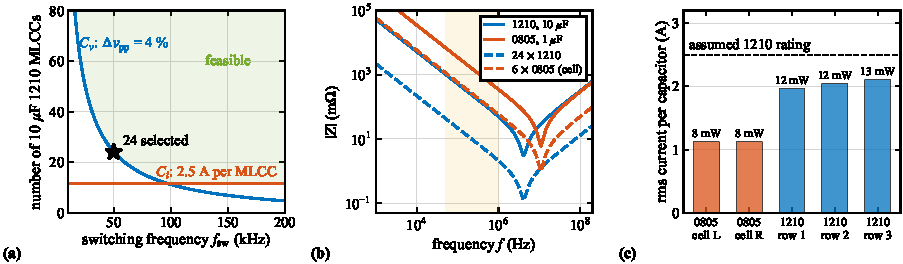
\includegraphics[width=0.92\textwidth]{fig_dclink.pdf}
\caption{DC-link design of the building block. (a) Number of 10\,\uF{} 1210 MLCCs per leg against switching frequency, required for a 4\,\% peak-to-peak voltage ripple on a three-leg submodule bus ($C_v$, blue) and for an rms current of 2.5\,A per capacitor ($C_i$, red); the shaded area is feasible, the star marks the selected bank. (b) Impedance magnitude of single capacitors (solid) and of the bank and the local group of one cell (dashed) from the $C_\mathrm{eff}$--ESR--ESL model; the shaded band covers the switching frequency and its first harmonics. (c) RMS ripple current and loss per capacitor at the rated point, from the frequency-domain network of the Q3D board impedances and the capacitor models.}
\label{fig:dclink}
\end{figure*}

The division of the ripple current between the capacitor groups depends on their ESR and ESL and on the board copper between them, so it is computed with the frequency-domain network of Section~\ref{sec:loss}, in which every capacitor group is represented by its $C_\mathrm{eff}$, ESR and ESL (Fig.~\ref{fig:dclink}b). At the switching frequency the bank is the lower impedance and carries most of the ripple: 2.0--2.1\,A$_\mathrm{rms}$ per 1210 capacitor, the third row slightly more, against 1.1\,A$_\mathrm{rms}$ per local 0805 capacitor (Fig.~\ref{fig:dclink}c). Above the self-resonance of the 1210 parts (about 4\,MHz) the local capacitors take over and supply the fast commutation transients. The total capacitor loss is \Pcap\,W per leg at the rated point, small compared with the other losses but concentrated in parts whose ripple current is already about 84\,\% of the assumed 2.5\,A rating; the bank is therefore designed close to both its voltage-ripple and its current limit at 50\,kHz.

%=========================================================================
\section{Parasitic and Gate-Loop Design}\label{sec:para}
%=========================================================================
\subsection{Power and gate loop}
The partial resistance and inductance matrix of the copper is extracted with Ansys Q3D at 100\,MHz, every component being represented by source and sink terminals on its pads, and is exported to LTspice as coupled inductors. Exciting both cells simultaneously gives a commutation-loop inductance of \LloopCu\,nH (copper) and \LloopEsl\,nH including the capacitor ESL per cell. Each transistor sees this loop; paralleling does not reduce the inductance, but each cell commutates half of the load current, so that the $di/dt$ per loop and thus the overshoot are halved. The value excludes the package inductance and routing details and is therefore a lower bound.

\begin{figure}[t]
\centering
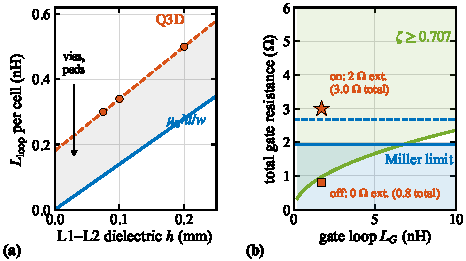
\includegraphics[width=\columnwidth]{fig_parasitics.pdf}
\caption{(a) Commutation-loop inductance per cell against the L1--L2 dielectric thickness $h$: Q3D (circles, linear fit dashed) and parallel-plate estimate $\mu_0hl/w$; the shaded difference is the fixed contribution of vias and pads. (b) Gate-resistor window per transistor in terms of the total gate resistance: damping bound at turn-on ($\zeta\geq0.707$, green) and Miller bound at turn-off (blue, solid for $V_\mathrm{th,min}$\,=\,0.8\,V, dashed for 1.1\,V); the markers are the selected external 2\,$\Omega$ (on) and 0\,$\Omega$ (off) resistors, i.e., 3.0 and 0.8\,$\Omega$ in total, at $L_G$\,=\,1.70\,nH.}
\label{fig:parasitics}
\end{figure}
The dielectric thickness $h$ between L1 and L2 is the dominant geometric parameter. Q3D gives \KqNHmm\,nH per millimetre of dielectric, close to the \KanNHmm\,nH/mm of the parallel-plate estimate $\mu_0hl/w$ used in~\cite{cooke2026,tran2025} (Fig.~\ref{fig:parasitics}a), plus a fixed \LfixNH\,nH from vias, pads and package that no dielectric reduction can remove. At 0.1\,mm (two-ply prepreg) the fixed part is already half of the loop.

The gate star gives \LgateOne\,nH per transistor. A side-mounted driver, as in a conventional single-row layout, would give 2.0 and 7.7\,nH to the near and far transistors (Q3D); the centre driver makes both branches equal by construction.

The common-source inductance $L_{CS}$ is the part of the source path that the gate loop and the power loop share. It is extracted with a combined Q3D model that contains the power loop, the gate star and its return: the Kelvin return leaves each QL source pad through a via and runs on L2 directly under the gate trace, in a slot of the dc$-$ plane, to the driver ground. With every loop described by its terminal currents, the gate-loop inductance is $L_G=\mathbf g^\mathsf{T}\mathbf L\,\mathbf g$ and the common-source inductance is the mutual term $L_{CS}=\mathbf g^\mathsf{T}\mathbf L\,\mathbf p$ between the gate loop $\mathbf g$ and the commutation loop $\mathbf p$ of the same cell. The Kelvin layout gives $L_{CS}$\,=\,\LcsKel\,nH, equal in both cells, and $L_G$\,=\,\LgateCs\,nH, which confirms the gate-star extraction; the coupling of a gate loop to the commutation loop of the other cell is only \MgateOther\,nH. At the turn-on $di/dt$ of about \DidtCell\,A/ns per transistor, $L_{CS}$ still induces about 0.8\,V of negative feedback in the gate loop, but equally in both transistors, so that it slows rather than unbalances the switching (Fig.~\ref{fig:sharing}). If the driver ground is instead connected to the dc$-$ plane next to the driver, the shared path grows to \LcsNoK\,nH. Table~\ref{tab:para} collects the extracted parasitics and the gate-drive parameters used in the circuit simulations.

\begin{table}[t]
\centering
\caption{Extracted Parasitics and Gate-Drive Parameters}
\label{tab:para}
\setlength{\tabcolsep}{3pt}
\resizebox{\columnwidth}{!}{%
\begin{tabular}{@{}llr@{}}
\toprule
\multicolumn{3}{@{}l}{\textbf{Power loop (Q3D, 100\,MHz)}} \\
$L_\mathrm{loop}$ per cell, copper / with MLCC ESL & BB\_PL & \LloopCu\,/\,\LloopEsl\,nH \\
ESL per MLCC, 1210 / 0805 & assumed & 0.50\,/\,0.48\,nH \\
\midrule
\multicolumn{3}{@{}l}{\textbf{Gate loop (Q3D, 100\,MHz)}} \\
$L_G$ per transistor (gate and Kelvin return) & BB\_CS & \LgateCs\,nH \\
$L_{CS}$, Kelvin via in the source pad & BB\_CS & \LcsKel\,nH \\
$L_{CS}$, driver ground on the dc$-$ plane & BB\_CS\_noK & \LcsNoK\,nH \\
Gate loop to power loop of the other cell & BB\_CS & \MgateOther\,nH \\
Mutual between the two gate loops & BB\_CS & \MgateGate\,nH \\
\midrule
\multicolumn{3}{@{}l}{\textbf{Gate resistances}} \\
$R_\mathrm{g,on}$ / $R_\mathrm{g,off}$ (external) & selected & 2\,/\,0\,$\Omega$ \\
$R_\mathrm{pu}$ / $R_\mathrm{pd}$ (driver output) & model & 0.6\,/\,0.2\,$\Omega$ \\
$R_\mathrm{G,int}$ (EPC2361) & datasheet & 0.4\,$\Omega$ \\
$R_{G,\mathrm{on}}$ / $R_{G,\mathrm{off}}$ total per transistor & & 3.0\,/\,0.8\,$\Omega$ \\
\bottomrule
\end{tabular}}
\end{table}

\subsection{Gate resistors and current sharing}
Treating the gate loop as a series RLC with $C_\mathrm{iss}$ gives a lower bound for the turn-on resistance, $R_{G,\mathrm{on}}\geq2\zeta\sqrt{L_G/C_\mathrm{iss}}$, and the Miller current an upper bound for the turn-off resistance, $R_{G,\mathrm{off}}\leq V_\mathrm{th}/(C_\mathrm{rss}\,dv/dt)$~\cite{tran2025} (Fig.~\ref{fig:parasitics}b). Inside this window, an LTspice sweep with the extracted parasitics at 160\,A selects external resistors of $R_\mathrm{g,on}/R_\mathrm{g,off}$\,=\,\RgOn/\RgOff\,$\Omega$, i.e., 3.0/0.8\,$\Omega$ in total with the 0.4\,$\Omega$ internal gate resistance and the 0.6/0.2\,$\Omega$ driver pull-up/pull-down (the pull-down shared by the two transistors): below 2\,$\Omega$ the high-side overshoot exceeds 90\,V (112\,V at 0.5\,$\Omega$), above it $E_\mathrm{on}$ rises. The peak $V_\mathrm{DS}$ is \VdsH\,V and \VdsL\,V for the high and low side, and the switching speeds are \DvdtOn\ and \DvdtOff\,V/ns at turn-on and turn-off. The off-state bump of the high-side gate is \VgsBump\,V, above the minimum threshold of 0.8\,V. It is the Miller charge of the held-off transistor divided onto its gate--source capacitance, $\Delta v_\mathrm{GS}\approx Q_\mathrm{GD}/C_\mathrm{GS}\approx\BmpDivider$\,V, because the hold-off path ($R_{G,\mathrm{off}}C_\mathrm{iss}\approx2.9$\,ns, $L_G/R_{G,\mathrm{off}}\approx2$\,ns) is as slow as the 4--6\,ns voltage transition. The bump is therefore almost independent of the load current (0.95--0.99\,V from 10 to 157\,A), of the bus voltage (\BmpFortyEight, \BmpSixty{} and \BmpSeventyFive\,V at 48, 60 and 75\,V) and of the driver pull-down resistance; it lasts about 2\,ns above 0.8\,V and does not cause channel conduction in the model even for a threshold of 0.6\,V. For margin in hardware, the final design uses a $-1$\,V off-state voltage, which the dual-channel isolated driver provides with a split +5/$-$1\,V supply referenced to the Kelvin source of each star: the peak gate voltage falls to \BmpNegOneSF\,V at 75\,V, the undershoot stays at $-2.3$\,V, inside the $-4$\,V rating, and the leg efficiency changes by only 0.01\,\% (a $-2$\,V bias brings the undershoot to \VgsMinNegTwo\,V, and a 2\,nF external gate--source capacitor reduces the peak only to \BmpCTwoSF\,V at 21\,\% higher $E_\mathrm{on}$).

Applied to the complete building block with the extracted parasitics, the symmetric layout of Section~\ref{sec:layout} (Fig.~\ref{fig:sharing}) leaves the two paralleled transistors with 78.53 and 78.63\,A at turn-off, i.e., a dynamic imbalance below 0.1\,\%.

%=========================================================================
\section{Switching Energies and Slow Switching}\label{sec:sw}
%=========================================================================
With the selected resistors, one switch position dissipates $E_\mathrm{on}$\,=\,\LcEonPk\,\textmu J and $E_\mathrm{off}$\,=\,\LcEoffPk\,\textmu J at \Ipk\,A. The turn-on energy consists of a current-independent part of \LcEonZero\,\textmu J, of the order of $Q_\mathrm{oss}V$, and an overlap part that follows $V^2I/(2\,dv/dt)$ within a few percent. The turn-off energy is almost independent of current: the gate is discharged through about 0.8\,$\Omega$ faster than the load current can move the output charge, so the channel is off before $V_\mathrm{DS}$ rises, the voltage rises at $dv/dt\approx I/C_\mathrm{oss,tot}$ (\SlowCoss\,nF), and most of the 7--8\,\textmu J measured at the device terminals is energy stored in $C_\mathrm{oss}$.

A motor-friendly design may slow the switching with larger gate resistors. Fig.~\ref{fig:slow} compares six resistor pairs simulated with the full building-block model. The turn-off becomes channel-controlled only when the gate removes the Miller charge more slowly than the load current moves the output charge, i.e.\ for
\begin{equation}
R_\mathrm{g,off,tot}>R_\mathrm{crit}=\frac{V_\mathrm{pl}\,Q_\mathrm{oss,tot}}{I\,Q_\mathrm{GD}},
\label{eq:rcrit}
\end{equation}
which gives about 1.5\,$\Omega$ at 139\,A and 7\,$\Omega$ at 30\,A ($V_\mathrm{pl}\approx2$\,V, $Q_\mathrm{GD}$\,=\,3.8\,nC). Above $R_\mathrm{crit}$ the voltage term of the classical overlap formula predicts $E_\mathrm{off}$ within about 10\,\%, whereas the additional current-fall term $I^2V/(2\,di/dt)$ overestimates it by a factor of 1.8; below $R_\mathrm{crit}$ the formula overestimates the loss by a factor of two. At turn-on, the $di/dt$ term is needed only when the gate resistance makes the current rise a separate, slow phase (10\,$\Omega$).

\begin{figure*}[t]
\centering
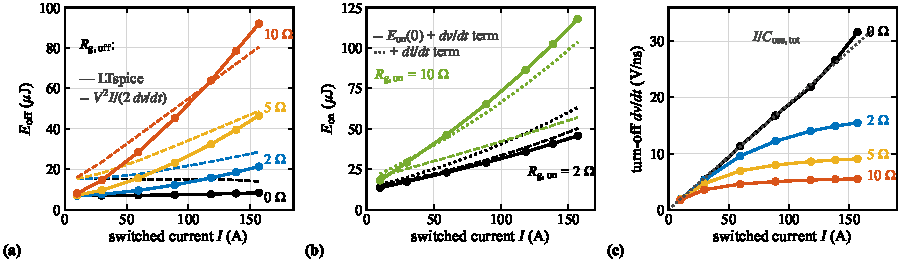
\includegraphics[width=0.92\textwidth]{fig_switching.pdf}
\caption{Switching energies per switch position of the building block with slow switching (LTspice with the Q3D parasitics, 75\,V, $R_\mathrm{g,on}$ and $R_\mathrm{g,off}$ external resistances). (a) Turn-off energy (solid) and voltage-overlap estimate $V^2I/(2\,dv/dt)$ with the simulated $dv/dt$ (dashed) for $R_\mathrm{g,off}$\,=\,0, 2, 5 and 10\,$\Omega$; the estimate fails below the critical resistance~\eqref{eq:rcrit}. (b) Turn-on energy for $R_\mathrm{g,on}$\,=\,2 and 10\,$\Omega$ against the current-independent part $E_\mathrm{on}(0)$ plus the voltage-overlap term (dashed) and plus the current-overlap term (dotted). (c) Turn-off $dv/dt$ against the load-driven limit $I/C_\mathrm{oss,tot}$ (dotted): without external resistance the voltage rise is set by the load current, with 5--10\,$\Omega$ by the gate.}
\label{fig:slow}
\end{figure*}


Two consequences follow for the drive design. First, $R_\mathrm{g,on}$\,=\,10\,$\Omega$ mainly slows the current rise: the turn-on $dv/dt$ falls only from 13 to 11\,V/ns while $E_\mathrm{on}$ rises 2.5 times; the turn-off $dv/dt$ is controlled by $R_\mathrm{g,off}$ only above $R_\mathrm{crit}$. Second, the same $R_\mathrm{g,off}$ holds the complementary transistor off, and its gate bump rises from 0.99 to 1.29\,V; slowing the turn-off therefore requires a separate low-impedance hold-off path. At 50\,kHz the leg efficiency falls from \SlEtaBase\,\% for the selected 2/0\,$\Omega$ pair to \SlEtaOffFive, \SlEtaOnTen{} and \SlEtaBoth\,\% for 2/5, 10/2 and 10/10\,$\Omega$, so that the fully slowed design misses the efficiency target.

%=========================================================================
\section{Losses Including Frequency-Dependent PCB Copper}\label{sec:loss}
%=========================================================================
The leg loss is evaluated for a sinusoidal current with continuous pulse-width modulation, for which conduction, switching and dead-time losses are identical for sinusoidal and space-vector modulation. With synchronous conduction, the high- and low-side transistors also share the loss equally for any modulation index and power factor, since $\overline{d\,i^2}=\overline{i^2}/2$.

The PCB copper loss is usually computed with dc resistances. The dc-link current of a phase leg, however, contains about 29\,A$_\mathrm{rms}$ at the switching frequency and its harmonics, which circulates between the MLCC bank and the cells. A Q3D frequency sweep from 1\,kHz to 100\,MHz shows that the branch resistances are already 1.5 times their dc value at 50\,kHz and 3 times at 500\,kHz (Fig.~\ref{fig:loss}a), because the current crowds onto the facing plane surfaces and the lowest-inductance paths. The board is therefore solved as a frequency-domain network of the Q3D $R(f)$ and $L(f)$ matrices, the capacitor groups and the dc-supply impedance, excited by the switched transistor currents at every harmonic of the modulated waveforms:
\begin{equation}
P_\mathrm{Cu}=\sum_h\tfrac12\,\mathbf I_h^\mathsf{H}\,\mathbf R(f_h)\,\mathbf I_h .
\end{equation}
The load-frequency part reproduces the dc estimate (\Pcu\,W); the switching harmonics add \PcuHf\,W at the rated point and up to \PcuHfLowM\,W at low modulation index, where the ripple current is largest. The same network gives an MLCC loss of \Pcap\,W.

\begin{figure*}[t]
\centering
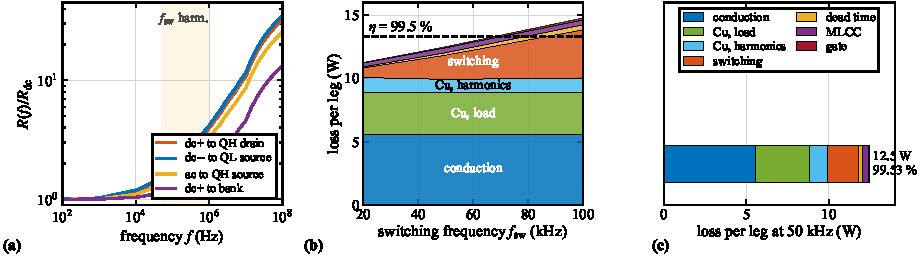
\includegraphics[width=0.92\textwidth]{fig_losses.pdf}
\caption{Losses of the building block at the rated point (75\,V, 100\,A$_\mathrm{rms}$, $M$\,=\,1, typical $R_\mathrm{DS(on)}$ at 100\,$^\circ$C). (a) Q3D resistance of the main board branches against frequency, normalized to the dc value; the shaded band covers the switching frequency and its first harmonics. (b) Loss per leg against switching frequency with the efficiency target. (c) Loss breakdown at 50\,kHz; conduction and copper loss together account for about 80\,\%.}
\label{fig:loss}
\end{figure*}
Fig.~\ref{fig:loss}(b) and~(c) show the resulting loss breakdown. At 50\,kHz the leg dissipates \Ptot\,W (\Eta\,\%): \PcondTyp\,W conduction, \PcuTot\,W copper, \Psw\,W switching, \Pdead\,W dead time and \Pcap\,W in the capacitors. Conduction and copper account for about 80\,\% of the loss, so cooling and copper design matter more than switching speed at this frequency, which is why the gate resistors could be selected for robustness. The 99.5\,\% target holds up to about \Fmax\,kHz; at 100\,kHz the efficiency is \EtaHundred\,\%, and with the maximum on-resistance the target is missed already at 50\,kHz (\EtaWorst\,\%). Without the switching-harmonic copper term, the same design would have appeared to reach 99.50\,\% at 100\,kHz.

The dc link of Section~\ref{sec:dclink} adds \Pcap\,W, and its size, not the transistors, bounds the useful switching frequency from the density point of view above about \Fcross\,kHz.

%=========================================================================
\section{Thermal Design}\label{sec:thermal}
%=========================================================================
A steady-state conduction model is built in Ansys Icepak from the same geometry. The board is an anisotropic equivalent of FR-4 and copper (in-plane 55\,W/mK, through-plane 0.36\,W/mK, 3.5\,W/mK in the cell regions with via arrays); each transistor is a 1.9\,W source with a junction-to-case resistance of 0.2\,K/W to the top and a junction-to-board resistance of 1.5\,K/W; a 0.5\,mm gap pad (1.9\,K/W per device) and aluminium pedestals connect the transistors to a 3\,mm aluminium plate held at 60\,$^\circ$C (liquid cold plate). The board copper loss (4.4\,W), the capacitor losses and the driver loss are applied as volumetric sources.

\begin{figure*}[t]
\centering
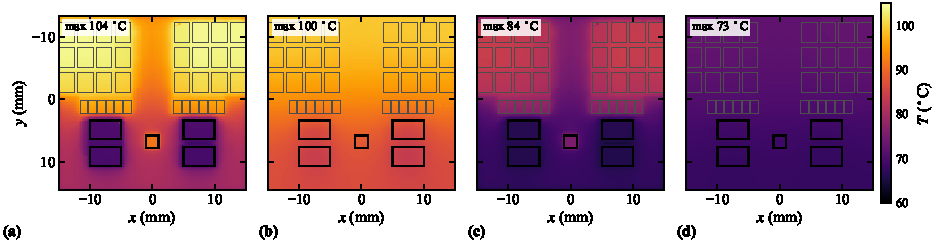
\includegraphics[width=0.86\textwidth]{fig_thermal.pdf}
\caption{Icepak temperature maps at the rated point (50\,kHz) in the device layer ($z$\,=\,2.0\,mm, including the air between components) and the board mid-plane. (a), (b) Cold plate on the transistors only. (c), (d) Additional bottom-side gap pad (3\,W/mK) to a second plate at 60\,$^\circ$C. Outlines: transistors, MLCCs and driver.}
\label{fig:thermal}
\end{figure*}

With the cold plate on the transistors only, the junctions stay at \ThFetTop\,$^\circ$C, 7\,K above a per-device estimate, because the transistors also conduct the heat of the board. The board itself, however, reaches \ThPcbTop\,$^\circ$C in the capacitor bank, where the 1210 capacitors reach \ThCapTop\,$^\circ$C and the driver \ThDrvTop\,$^\circ$C (Fig.~\ref{fig:thermal}): its copper loss, larger than the loss of each transistor, has no path to the cold plate other than laterally through the board and upwards through the transistors. A bottom-side gap pad to a second plate lowers the board maximum to \ThPcbBoth\,$^\circ$C and the junctions to \ThFetBoth\,$^\circ$C. Since the model distributes the copper loss over the board thickness and neglects convection, the absolute board temperatures are conservative; the conclusion that a low-voltage, high-current building block needs a cooling path for its board copper is not.

%=========================================================================
\section{Integration and Machine Side}\label{sec:integ}
%=========================================================================
\begin{figure*}[t]
\centering
\subfloat[]{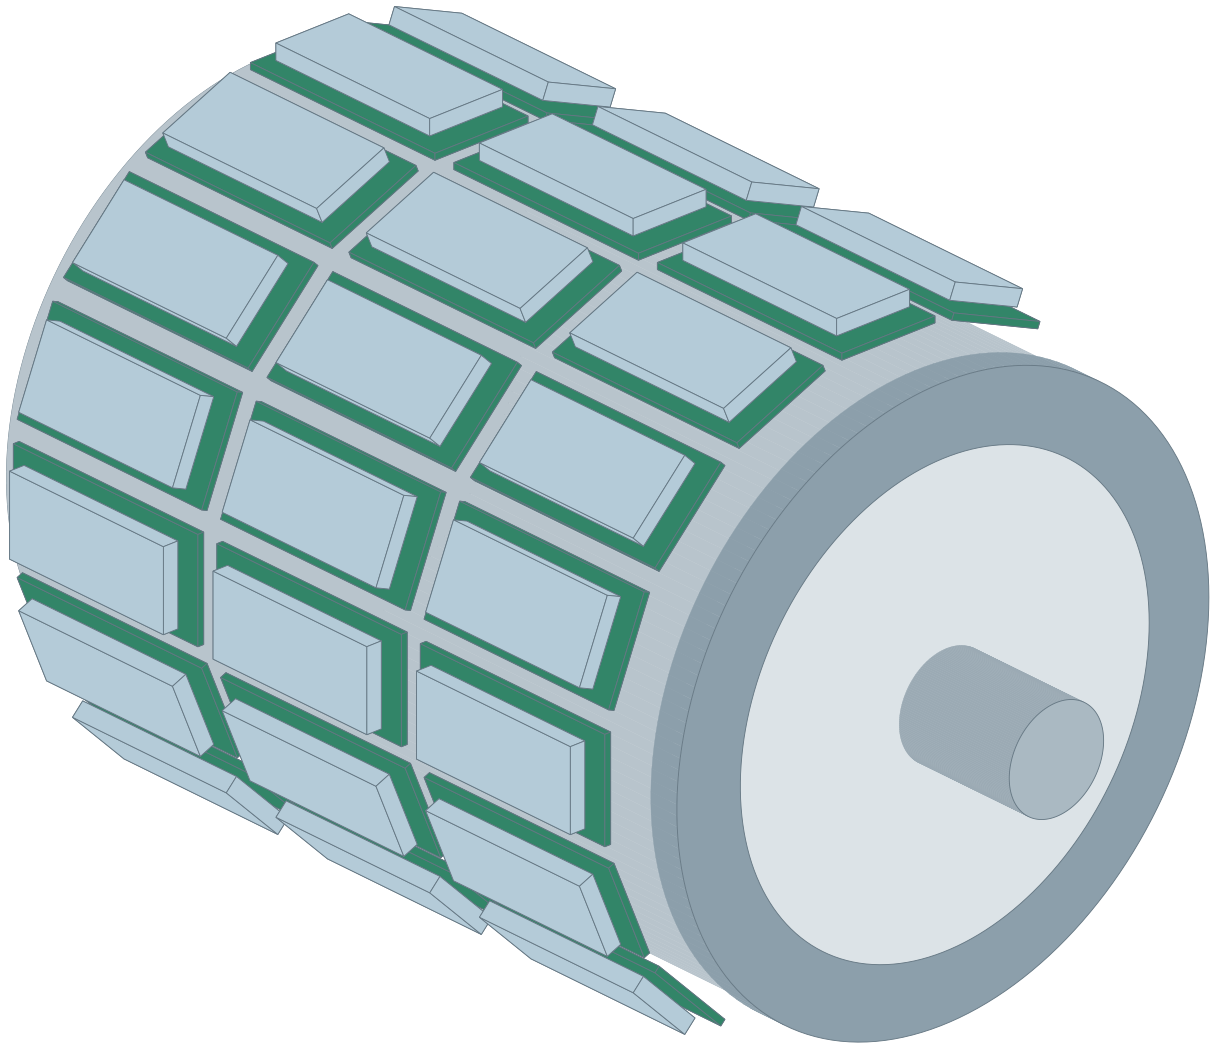
\includegraphics[height=4.6cm]{motor_integration.png}}\hfill
\subfloat[]{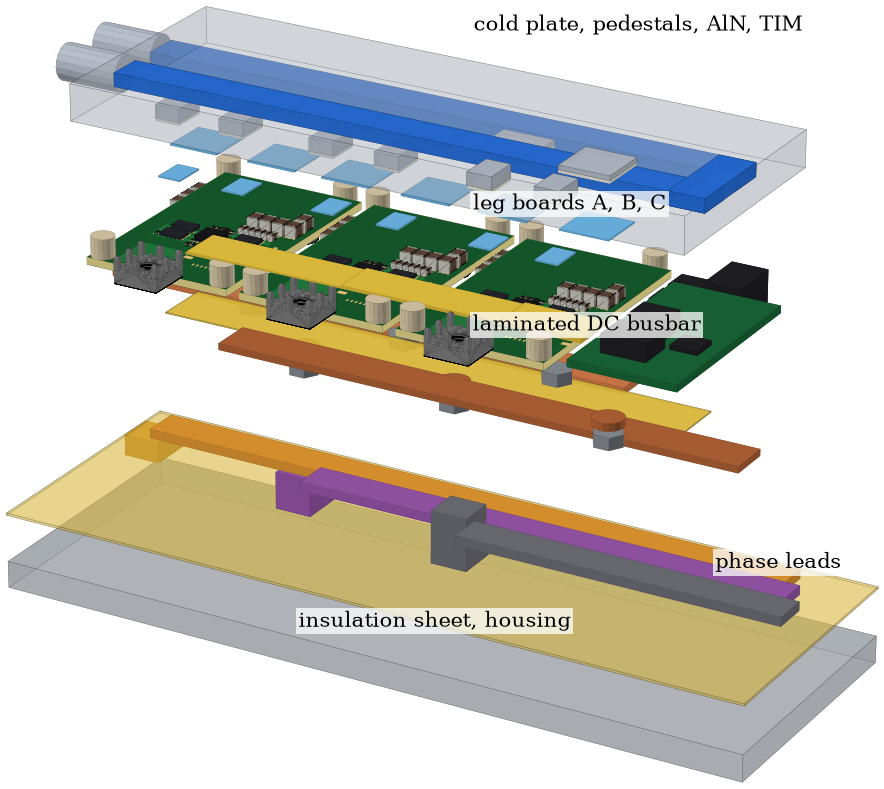
\includegraphics[height=4.6cm]{cell_exploded.png}}\hfill
\subfloat[]{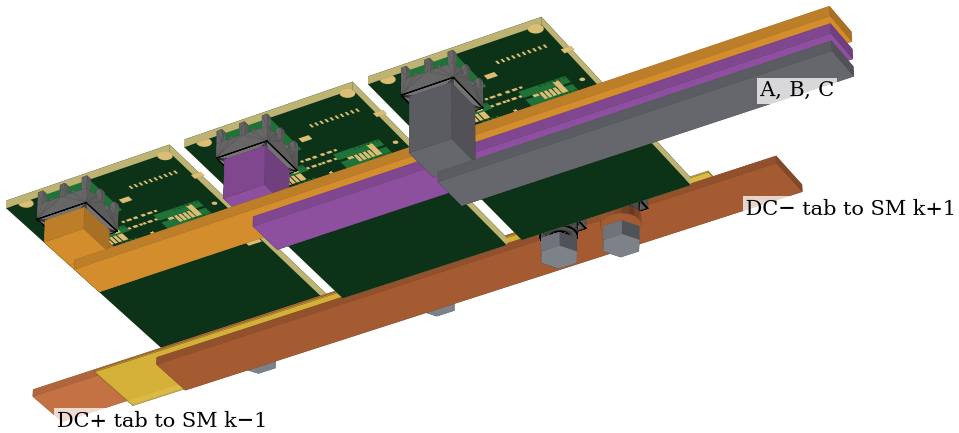
\includegraphics[height=3.4cm]{cell_bottom.png}}
\caption{Machine-integrated SPB drive. (a) Concept: 16 cells (submodules) around the housing of a radial-flux machine, each with three leg building blocks along the axial direction, 48 legs in total (conceptual geometry). (b) Exploded view of one cell: liquid cold plate (transparent) with U-shaped channel and pedestals tipped with AlN insulators and thermal pads, the three leg boards with insulated standoffs, the laminated dc busbar, the phase leads and the insulation sheet above the housing; the aux/control board is at the end of the cell. (c) Cell seen from below: the busbar connects the dc terminals of the three legs and ends in series tabs to the neighboring cells; each phase lead leaves its ac terminal at its own depth and runs axially to the end winding.}
\label{fig:integ}
\end{figure*}

\subsection{Cell assembly}
For the machine-integrated drive, the three legs of a submodule are mounted along the axial direction under one liquid cold plate, and the 16 cells are arranged around the housing (Fig.~\ref{fig:integ}a). The leg board is extended by a dc terminal zone and a tab for the ac terminal and the gate-drive connector (33\,$\times$\,52.7\,mm including I/O, with the power stage unchanged), so that one cell is about 132\,mm long and 53\,mm wide and the 16 cells fit a housing of about 300\,mm diameter. Every cell floats at up to the full stack voltage against the grounded cold plate. Instead of a thick insulating gap pad, the plate carries pedestals over each transistor pair and each capacitor bank, tipped with 0.63\,mm AlN insulators and only a thin compliant pad to the parts (Fig.~\ref{fig:integ}b); the AlN adds about 0.25\,K/W per transistor, compared with 1.9\,K/W for the 0.5\,mm gap pad of Section~\ref{sec:thermal}, and the insulator overhang provides the creepage path. With about 38\,W per cell, the coolant temperature rises by less than 1\,K along a cell at 1\,L/min, so the cells can be fed in parallel from a ring manifold, before the coolant enters the stator jacket.

\begin{figure}[t]
\centering
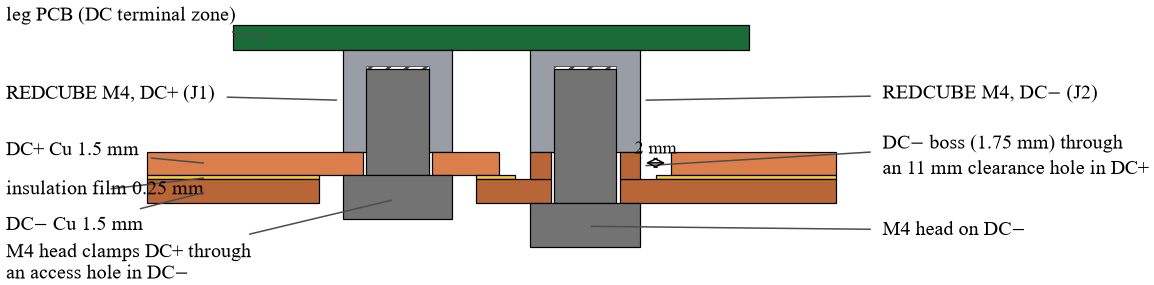
\includegraphics[width=\columnwidth]{busbar_section.png}
\caption{Section of the laminated busbar through the dc terminals of one leg: 1.5\,mm DC+ copper on the DC+ terminal, 0.25\,mm insulation film, 1.5\,mm DC$-$ copper reaching its terminal with a boss through an 11\,mm clearance hole; the DC+ screw is reached through an access hole in the DC$-$ layer.}
\label{fig:busbar}
\end{figure}
The dc terminals of the three legs lie on one edge of the boards and are bolted to a laminated busbar under the cell (Figs.~\ref{fig:integ}c and~\ref{fig:busbar}). Its two layers overlap along the whole cell, which keeps the inductance between the legs low, and its ends form the series connections to the neighboring cells, which carry the bus current of about 125\,A. Each ac terminal carries an 8\,$\times$\,2\,mm copper lead to the end winding. A small aux/control board at the end of each cell is supplied from the cell's own dc link (a 75\,V buck and isolated 6\,V supplies for the three high-side drivers), so that no auxiliary supply has to be isolated for the full stack voltage; the cell communicates with the central controller over optical fibre and measures the cell voltage, the board temperatures and the phase currents.

\subsection{Machine-side couplings}
The machine is not designed yet, but it closes the design loop of Fig.~\ref{fig:flow} through three quantities. First, the number of submodules equals the number of three-phase winding sets, so the voltage class of Section~\ref{sec:vclass} fixes $N$ and the turns per set; conversely, a machine with a different number of sets changes $V_m$ and the voltage utilization of the transistors. Second, the switching frequency is set by the ripple of each winding set,
\begin{equation}
\Delta i_\mathrm{pp,max}\approx\frac{V_m}{4\,L_\sigma f_\mathrm{sw}},
\label{eq:ripple}
\end{equation}
where $L_\sigma$ is the leakage inductance of one set. If $L_\sigma$ scales with the square of the turns, splitting a winding into $N$ sets reduces $L_\sigma$ by $N^2$ and $V_m$ by $N$, so that at a given $f_\mathrm{sw}$ the ripple of each set grows with $N$. A larger number of submodules therefore requires a higher switching frequency, interleaved carriers between the submodules to cancel the ripple in the air-gap flux~\cite{bringezu2020}, or more leakage inductance; the optimum $f_\mathrm{sw}$ follows from the sum of the inverter losses (Fig.~\ref{fig:loss}b) and the ripple losses of the machine~\cite{cooke2024}. Third, the winding sees voltage steps of only $V_m$ instead of the full bus voltage, so that the turn-to-turn insulation stress is small even at 10--30\,V/ns, while the insulation of each set to the stator and between sets must still withstand the stack voltage. Finally, the drive and the machine share the coolant and the space at the end winding, which sets the cold-plate width, the routing of the 48 phase leads and the order of the coolant flow.

%=========================================================================
\section{Discussion and Future Work}
%=========================================================================
\begin{table}[t]
\centering
\caption{Comparison With Paralleled-GaN Half Bridges}
\label{tab:sota}
\setlength{\tabcolsep}{2.5pt}
\resizebox{\columnwidth}{!}{%
\begin{tabular}{@{}lllll@{}}
\toprule
Work & Devices/switch & Rating / test & $L_\mathrm{loop}$ & Layout \\
\midrule
\cite{lu2017} & 4\,$\times$\,650\,V & 400\,V/240\,A DPT & 0.7\,nH & 6-layer PCB \\
\cite{tran2025} & 4\,$\times$\,100\,V & 48\,V/328\,A DPT & 1.14\,nH & IMS hybrid \\
\cite{cooke2026} & 8\,$\times$\,200\,V & 120\,V/155\,A, 100\,kHz & 0.34\,nH$^\ast$ & PCB, symm.\ gate \\
\cite{wattenberg2023} & 8\,$\times$\,100\,V & 48\,V/125\,A$_\mathrm{rms}$ & -- & butterfly PCB \\
\cite{novo2024} & 4\,$\times$\,650\,V & 350\,A$_\mathrm{rms}$ WLTP & 3.9\,nH & PCB module \\
\cite{zou2025} & 3\,$\times$\,650\,V & 400\,V, 100\,kW & 6.4\,nH & PCB + Cu blocks \\
This work & 2\,$\times$\,100\,V & 75\,V/141\,A (design) & 0.37\,nH/cell & mirrored cells \\
\bottomrule
\multicolumn{5}{@{}l}{\footnotesize $^\ast$analytical estimate}
\end{tabular}}
\end{table}

Compared with the reviewed paralleled-GaN half bridges (Table~\ref{tab:sota}), whose commutation loops range from 0.34 to 6.4\,nH, and up to 11\,nH in a commercial module~\cite{brothers2019}, the proposed block reaches \LloopEsl\,nH per cell with two loops in parallel, and its symmetric gate drive removes the dominant sharing mechanisms. The analysis identifies five limits that guide the next iteration: the voltage margin, since with an overshoot of about 11\,V a 75\,V submodule reaches about 101\,V at 20\,\% above its nominal voltage, so that a regulated submodule voltage or about 60\,V nominal ($N$\,=\,20) is needed; the copper loss, which can be reduced by about 2\,W with busbar contacts next to each cell and heavier inner layers, and further by placing more capacitance next to the cells to shorten the ripple path; the thermal path of the board; and the dc-link ripple on a shared submodule bus, which is at its limit.

All results in this paper are from analysis, finite-element extraction and circuit simulation. Experimental validation is future work: double-pulse tests at 75\,V and up to 160\,A, including the loop inductance from the ringing frequency and the per-transistor currents, continuous operation for efficiency and thermal-image based sharing checks~\cite{cooke2026}, measurement of the capacitor impedances, and finally an SPB submodule driving a multiphase machine, where the trade-off between inverter and machine losses will set the switching frequency~\cite{cooke2024}.

%=========================================================================
\section{Conclusion}
%=========================================================================
A design procedure for the building block of stacked polyphase bridge converters has been presented and applied to a 1200\,V, 150\,kW traction inverter. The device time constant $R_\mathrm{DS(on)}C_\mathrm{oss,tr}$ selects the 100\,V class and EPC2361, hence 16 submodules of 75\,V; a star-connected driver per pair of paralleled transistors fixes the layout; and the loss gain from one to two devices per switch, compared with the small gain and the doubled driver count for three, sets two devices per switch. The dc link of 24 1210 and 12 0805 MLCCs per leg is limited by voltage ripple and ripple current at about the same frequency. The block reaches \LloopEsl\,nH per cell and \Eta\,\% efficiency at 50\,kHz on 8.5\,cm$^2$. The design shows that the switching harmonics of the dc-link current add about one third to the dc copper loss of the board, that the overlap loss formula applies to a GaN turn-off only above the critical gate resistance~\eqref{eq:rcrit}, and that the board copper, rather than the transistors, sets the thermal design of a low-voltage, high-current building block.

\begin{thebibliography}{99}
\bibitem{norrga2013} S.~Norrga, L.~Jin, O.~Wallmark, A.~Mayer, and K.~Ilves, ``A novel inverter topology for compact EV and HEV drive systems,'' in \emph{Proc. IECON}, 2013, pp. 6590--6595.
\bibitem{jin2014} L.~Jin, S.~Norrga, O.~Wallmark, and M.~Nikouei Harnefors, ``Control and modulation of the stacked polyphase bridges inverter,'' in \emph{Proc. IEEE ECCE}, 2014.
\bibitem{jin2017} L.~Jin, S.~Norrga, O.~Wallmark, and N.~Apostolopoulos, ``Modulation and power losses of a stacked polyphase bridge converter,'' \emph{IEEE J. Emerg. Sel. Topics Power Electron.}, vol.~5, no.~1, pp. 409--418, Mar. 2017.
\bibitem{jin2016} L.~Jin, S.~Norrga, and O.~Wallmark, ``Analysis of power losses in power MOSFET based stacked polyphase bridges converters,'' in \emph{Proc. IPEMC-ECCE Asia}, 2016.
\bibitem{nikouie2017tpel} M.~Nikouie, O.~Wallmark, L.~Jin, L.~Harnefors, and H.-P.~Nee, ``DC-link stability analysis and controller design for the stacked polyphase bridges converter,'' \emph{IEEE Trans. Power Electron.}, vol.~32, no.~2, pp. 1666--1674, Feb. 2017.
\bibitem{nikouie2017} M.~Nikouie, H.~Zhang, O.~Wallmark, and H.-P.~Nee, ``A highly integrated electric drive system for tomorrow's EVs and HEVs,'' in \emph{Proc. IEEE SPEC}, 2017.
\bibitem{zhang2014} H.~Zhang, O.~Wallmark, M.~Leksell, S.~Norrga, M.~Nikouei Harnefors, and L.~Jin, ``Machine design considerations for an MHF/SPB-converter based electric drive,'' in \emph{Proc. IECON}, 2014.
\bibitem{bringezu2020} T.~Bringezu and J.~Biela, ``Comparison of optimized motor-inverter systems using a stacked polyphase bridge converter combined with a 3-, 6-, 9-, or 12-phase PMSM,'' in \emph{Proc. EPE ECCE Europe}, 2020.
\bibitem{bringezu2023} T.~Bringezu and J.~Biela, ``Control of a 9-phase PMSM with stacked polyphase bridge converter including dc source impedance,'' in \emph{Proc. EPE ECCE Europe}, 2023.
\bibitem{verkroost2024} L.~Verkroost, F.~De~Belie, L.~Faria da Rocha, P.~Keim Olsen, P.~Sergeant, and H.~Vansompel, ``Multi-agent control scheme for power distribution in a multi-three-phase motor drive fed by a stacked polyphase bridges converter,'' \emph{IEEE Trans. Energy Convers.}, vol.~39, no.~4, pp. 2568--2580, Dec. 2024.
\bibitem{brothers2019} J.~A.~Brothers and T.~Beechner, ``GaN module design recommendations based on the analysis of a commercial 3-phase GaN module,'' in \emph{Proc. IEEE ECCE}, 2019, pp. 4109--4116.
\bibitem{lu2017} J.~Lu and D.~Chen, ``Paralleling GaN E-HEMTs in 10\,kW--100\,kW systems,'' in \emph{Proc. IEEE APEC}, 2017, pp. 3049--3056.
\bibitem{tran2025} M.~T.~Tran \emph{et al.}, ``A high-performance GaN power module with parallel packaging for high-current and low-voltage traction inverter applications,'' \emph{IEEE J. Emerg. Sel. Topics Power Electron.}, vol.~13, no.~1, pp. 1188--1209, Feb. 2025.
\bibitem{musumeci2022} S.~Musumeci, V.~Barba, and M.~Palma, ``GaN-based low-voltage inverter for electric scooter drive system,'' in \emph{Proc. AEIT Int. Annu. Conf.}, 2022.
\bibitem{wattenberg2023} M.~Wattenberg, O.~G.~Lorenz, and J.~Sanchez, ``A multi-kilowatt low-profile GaN inverter for light electric vehicles and high-power tools,'' in \emph{Proc. IEEE APEC}, 2023, pp. 1443--1450.
\bibitem{cooke2026} M.~W.~J.~Cooke and D.~J.~Rogers, ``120\,V, 155\,A traction inverter using eight parallel GaN HEMTs,'' 2026.
\bibitem{zou2025} M.~Zou \emph{et al.}, ``Systematic efficiency-density co-optimization of 100\,kW GaN traction inverter: methodology and integration,'' \emph{IEEE Trans. Power Electron.}, vol.~40, no.~11, pp. 16281--16299, Nov. 2025.
\bibitem{rahman2025} M.~D.~Rahman \emph{et al.}, ``Design and evaluation of a 650\,V, 300\,A GaN-based power module with integrated drivers and ultra-low inductance layout,'' in \emph{Proc. IEEE WiPDA}, 2025.
\bibitem{novo2024} D.~Novo \emph{et al.}, ``Development and testing of GaN power modules for EV traction inverters,'' in \emph{Proc. CIPS}, 2024, pp. 692--698.
\bibitem{rohner2024} G.~Rohner, J.~Huber, S.~Miri\'c, and J.~W.~Kolar, ``Comparative evaluation of three-phase three-level flying capacitor and stacked polyphase bridge GaN inverter systems for integrated motor drives,'' \emph{Electronics}, vol.~13, no.~7, Art.~no.~1259, 2024, doi: 10.3390/electronics13071259.
\bibitem{cooke2024} M.~Cooke and D.~J.~Rogers, ``Effect of switching frequency on efficiency in wide bandgap based drive systems,'' in \emph{Proc. IEEE WiPDA}, 2024.
\end{thebibliography}

\end{document}
